\section{Konzepte der Messunsicherheitsfortpflanzung (M.U.F.)}

% 1 Fortpflanzung für lineare Modelle
% 2 Überdeckungsintervall 
% 3 Kombinierte Standardabweichung 
%   (Sattherthwaite) 
% 4 Erweiterungsfaktor 

In der Messtechnik geht es darum, indirekte Messgrößen über Beobachtungen von direkten
Messgrößen und über ein Schätzverfahren auf Basis eines Modells zu ermitteln.
In der ersten Vorlesung hatten wir dazu hervorgehoben, dass zu dem Modell zum einen
die mathematische Beschreibung des physikalischen Sachverhaltes gehört und zum anderen
die statistische Beschreibung von nicht deterministischem Verhalten, das in erster
Linie von nicht vorhersehbaren, kleinen Störeinflüssen und Auflösungsbegrenzungen
beim Beobachtungsvorgang verursacht wird, aber auch von dem physikalischen Vorgang, der
zu untersuchen ist, selber stammt, wie beispielsweise bei radioaktiven Zerfällen, Streuprozesse
atomarer Vorgänge oder bei biologischen Prozessen. Das nicht deterministische Verhalten, die
Stochastik, eines Prozesses wird mittels entsprechender Wahrscheinlichkeitsverteilungen modelliert.

Ein Messergebnis einer Größe $X$ wird deshalb statistisch mit Wahrscheinlichkeitsverteilungen ausgedrückt
\begin{itemize}
\item in Form einer Wahrscheinlichkeitsdichteverteilung
$$
p(X)
$$
oder
\item in Form der statistischen Momente, Erwartungswert $x$ und Varianz (bzw.\ deren Wurzel $\sigma_X$),
einer Wahrscheinlichkeitsdichteverteilung, zusammen mit einer Wahrscheinlichkeit $1-\alpha$
bzw.\ einem Quantil $k$
$$
x = \int X p(X) \operatorname d X, \quad
\sigma_X = \sqrt{\int (X-x)^2 p(X) \operatorname d X}, \quad k = P^{-1}(1-\alpha/2).
$$
\end{itemize}
Dreh- und Angelpunkt bei der Quantifizierung von Messgrößen ist die Vorgehensweise, wie ein entsprechendes
Messergebnis durch Modellbildung, Parameterschätzung und Bestimmung der Wahrscheinlichkeitsdichtefunktion
der Parameter gewonnen wird. Ein Messergebnis einer Größe $Y$ oder eines Größenvektors
$\mathbf{Y}$, die bzw.\ der \textsl{explizit} oder \textsl{implizit} von direkten
Messgrößen $\mathbf{X}$ abhängt, soll entsprechend ausgedrückt werden durch eine
Wahrscheinlichkeitsdichteverteilung $p(Y)$ bzw.\ durch den entsprechenden Erwartungswert $y$ und
die Wurzel aus der Varianz $\sigma_Y$ mit einem Quantil $k$, dem Erweiterungsfaktor, für
eine spezifizierte Wahrscheinlichkeit $1-\alpha$.

Wir kategorisieren die Modelle für indirekte Messgrößen
danach, ob sie univariat oder multivariat und ob sie explizit oder implizit sind:

\begin{center}
{\setlength{\extrarowheight}{4pt}%
\begin{tabular}{l||c|c|}
\arraycolsep=4pt\def\arraystretch{2}
 & univariat: $1$ indirekte Größe & multivariat: $M>1$ indirekte Größen \\[4pt]
\hline\hline
explizit & $Y = f(\mathbf{X})$ & $\mathbf{Y} = \vec f(\mathbf{X})$\\[4pt]
\hline
implizit & $f(Y,\mathbf{X})=0$ & $f(\mathbf{Y},\mathbf{X})=0$ oder
 $\vec f(\mathbf{Y},\mathbf{X})=0$\\[4pt]
\hline
\end{tabular}}
\end{center}

mit $\mathbf{X} = (X_1,\dots,X_N)^\mathsf{T}$ und $\mathbf{Y} = (Y_1,\dots,Y_M)^\mathsf{T}$.

Bei der linearen Regression beispielsweise haben wir, wie wir es in der zweiten Vorlesung
gelernt haben, die Regressoren und Regressanden als
\begin{enumerate}
\item gemeinsam ausgelesene (z.B.\ durch Triggerung zugeordnete) Beobachtungstupel
\begin{equation}
\boldsymbol (Y_{\mathrm{Regr}, j}, \mathbf{X}_j) \; = \; (Y_{\mathrm{Regr}, j}, X_{1,j}, \dots, X_{M,j})
\end{equation}
vorliegen mit $j = 1,\dots, J$ und $J$ für den Stichprobenumfang, so dass gemäß einem
zeitlichen Ablauf eine Veränderung aller Größen vorliegen kann,
\item ansonsten können die direkten Messgrößen in voneinander unabhängigen Experimenten
und damit im allgemeinen auch mit verschiedenen Stichprobenumfängen gewonnen werden.
\end{enumerate}

Der erstere Fall repräsentiert als direkte Größen
sowohl die Regressoren $\mathbf{X}$ als auch die Regressanden $Y_{\mathrm{Regr}}$
und als indirekte Messgrößen, die Modellparameter $\boldsymbol \theta \equiv \boldsymbol Y$.
Hier handelt es sich also hinsichtlich der Unsicherheitsfortpflanzung um ein
implizites, multivariates Problem, auch bei der univariaten, linearen Regression.
\begin{equation}
0 = f(\mathbf{Y},\mathbf{X}) \equiv f(\boldsymbol \theta,\mathbf{X})
= Y_{\mathrm{Regr}} - \sum_{i=1}^{M} \theta_i \, X_i
\label{implizitMultivariatRegre}
\end{equation}
Das \glqq Multivariate\grqq ~für die Unsicherheitsberechnung betrifft die indirekten
Messgrößen $\boldsymbol \theta \equiv \boldsymbol Y$, das \glqq Univariate\grqq ~für die
Regression betrifft den Regressanden $Y_{\mathrm{Regr}}$.

Fall zwei kann im allgemeinen so geartet sein, dass jede der direkten Größen in jeweils unabhängigen
Messvorgängen gewonnen wird, bei denen im allgemeinen unterschiedliche Stichprobenumfänge $J_i, J_k$ vorliegen
können und dann keine paarweise Zuordnung der einzelnen Beobachtungswerte $X_{i,j}$ zu $X_{k,l}$ für
$i \neq k$ vorliegt.

Bei dem expliziten, univariaten Fall
\begin{equation}
Y = f(\mathbf{X})
\label{explizitUnivariat}
\end{equation}
können die direkten Messgrößen als unkorrelierte unterschiedliche Stichproben vorliegen (Fall 2)
oder auch als gemeinsam getriggerte Tupel
\begin{equation}
\boldsymbol X_j \; = \; (X_{1,j}, \dots, X_{N,j})
\end{equation}
wie in Fall 1, aber dann nicht mit Regressionskoeffizienten als Modellparameter, sondern
mit der indirekten Größe explizit als Funktion von $(X_{1}, \dots, X_{N})$ gemäß
Gl.~(\ref{explizitUnivariat}).


Für eine internationale Vergleichbarkeit und den internationalen Handel ist es erforderlich,
dass die Verfahren zur Bestimmung von Messergebnissen möglichst einheitlich sind.
Für das gesetzliche Messwesen ist deshalb die international übereingekommene Richtlinie
zur Bestimmung von Messunsicherheiten bindend.
Die internationale Richtlinie zur Berechnung von Messunsicherheiten umfasst mehrere
Dokumente:
\begin{itemize}
\item JCGM 100:2008 GUM 1995 with minor corrections \textsl{Evaluation of measurement
data - Guide to the expression of uncertainty in measurement}; oftmals einfach mit \glqq GUM\grqq ~bezeichnet,
betrifft univariate und explizite Modelle, 
  \begin{itemize}
  \item die linear sind
  \begin{equation}
  Y = f(\mathbf{X}) = \sum_{i=1}^N c_i X_i
  \label{univarLinear}
  \end{equation}
  oder für die eine Linearisierung zulässig ist
  \begin{equation}
  Y = f(\mathbf{X})
  = \left. f(\mathbf{X}) \right|_{\bar{\mathbf{x}}} + 
    \sum_{i=1}^N \underbrace{\left. \frac{\partial f}{\partial X_i} \right|_{\bar{\mathbf{x}}}}_{c_i} \Delta X_i
  \label{univarTaylorLin}
  \end{equation}
  \item die Zufallsgrößen betreffen, deren Streuung (\textsl{dispersion}) normalverteilt oder
  $t$-verteilt ist.
  \end{itemize}
Hier wird die Varianz der indirekten Größe als lineare Funktion der Varianzen
der indirekten Größen modelliert, die Varianzen werden \glqq fortgepflanzt\grqq.\\
$\rightarrow$ Vorlesung 8
\begin{equation}
\operatorname{Var}(Y) = \sum_{i=1}^N \sum_{k=1}^N  c_i c_k \operatorname{Cov}(X_i, X_k)
\label{univarLinearFortpflanzung}
\end{equation}
\item JCGM 101:2008 \textsl{Evaluation of measurement
data - Supplement 1 to the Guide to the expression of
uncertainty in measurement - Propagation of distributions using a Monte Carlo method}; 
kurz mit \glqq GUM - supplement 1\grqq ~bezeichnet, betrifft
explizite und implizite, univariate Modelle,
  \begin{itemize}
  \item die sich nicht einfach linearisieren lassen 
  \item und/oder die sich nicht in einer geschlossenen analytischen Form darstellen lassen.
  \end{itemize}
Hier wird zu jeder direkten Messgröße eine Wahrscheinlichkeitsdichteverteilung vorgegeben.
Gemäß den jeweiligen Verteilungen wird eine große Stichprobe (ein großes \textsl{Sample}) 
$\mathbf{x}_1 = (x_{1,1},\dots,x_{N,1})^\mathsf{T}$, $\dots$, $\mathbf{x}_J = (x_{1,J},\dots,x_{N,J})^\mathsf{T}$
für die direkten Größen $\mathbf{X}$ per Zufallszahlengenerator erzeugt. Diese wird in das Modell $f$ gesteckt,
um eine Stichprobe
\begin{equation}
y_1 = f(x_{1,1},\dots,x_{N,1}), \dots, y_J = f(x_{1,J},\dots,x_{N,J})
\end{equation}
der indirekten Größe $Y$ zu gewinnen. Das Histogramm der Stichprobe der indirekten Größe liefert somit die
Wahrscheinlichkeitsdichteverteilung. Aus der sortierten Stichprobe nach der Art wie wir sie
für den Kolmogoroff-Smirnow-Test berechnet haben, gewinnen wir die kumulierte Wahrscheinlichkeitsverteilung
aus deren inverser Funktion das Überdeckungsintervall gewonnen werden kann.\\
$\rightarrow$ Vorlesung 10 und 11
\item JCGM 102:2011 \textsl{Evaluation of measurement data – Supplement 2 to the
Guide to the expression of uncertainty in measurement - Extension to any number of output quantities}
liefert die Verallgemeinerung der beiden Richtliniendokumente JCGM 100 und JCGM 101 für den multivariaten
Fall mit mehreren $M>1$ indirekten Größen, also einem Größenvektor $\mathbf{Y}$.
Hier wird dargelegt, wie man die Unsicherheit 
  \begin{itemize}
  \item bei linearen oder linearisierbaren Modellen
    mittels der Berechnung der Kovarianzen (in der Art wie wir es
    in Vorlesung 2 für die lineare Regression kennen gelernt haben)
  \item oder im Fall der nicht linearisierbaren und/oder komplexeren (oftmals impliziten) Modelle
    via Monte-Carlo-Berechnungen analog zu GUM-supplement 1
  \begin{equation}
  \mathbf{y}_1 = \vec f(x_{1,1},\dots,x_{N,1}), \dots, \mathbf{y}_J = \vec f(x_{1,J},\dots,x_{N,J})
  \end{equation}
  \item sowie für alle Fälle, ob uni- oder multivariat, ob explizit oder implizit, ob analytisch
    oder via Monte-Carlo-Verfahren unter Einbeziehung von {\`a} priori-Information mittels
    Bayesischen Methoden\\
    $\rightarrow$ Vorlesung 9
  \end{itemize}
ermittelt.
\item JCGM 103 CD 2018-10-04 \textsl{Guide to the expression of uncertainty in measurement
- Developing and using measurement models} behandelt in umfassender Weise die Problematik der
Modellentwicklung. Es gibt den Bereich physikalischer, deterministischer Prozesse,
den Bereich der nicht-deterministischen, physikalischen oder biologischen oder soziologischen
Prozesse. Ferner gibt es den Bereich der statistischen Modelle, die dazu dienen, nicht-deterministische
Anteile von Prozessen zu behandeln. Das JCGM 103 Dokument soll diese Dinge konzeptionell
für die Metrologie beleuchten. Es ist bisher ein Entwurf; das Kürzel CD steht für \textsl{committee draft}.
\item JCGM 104:2009 \textsl{Guide to the expression of uncertainty in measurement
- An introduction to the Guide to the expression of
uncertainty in measurement and related documents} liefert die Konzepte und Hintergründe zur
Unsicherheitsbestimmung. Dieses Dokument soll ein Verständnis für die Konzepte der
Wahrscheinlichkeitsdichteverteilungen im Zusammenhang mit der Bestimmung von Messunsicherheiten liefern.
\item JCGM 106:2012 \textsl{Evaluation of measurement data - The role of
measurement uncertainty in conformity assessment}. Im Rahmen der Vorlesungen zu Hypothesentests und
Ringvergleichen haben wir bereits gelernt, dass Messergebnisse zu vergleichen sind, und wie dies
gehandhabt wird. In der Qualitätssicherung ist die zentrale Aufgabe, gefertigte Bauteile mit den
vorgegebenen Daten der technischen Konstruktionszeichnung zu vergleichen hinsichtlich der Übereinstimmung,
also der Einhaltung von Toleranzgrenzen. Dies wird Konformitätsbewertung genannt und wird im
JCGM 106-Dokument behandelt.
\end{itemize}

Das historisch älteste Dokument JCGM~100, das für linearisierbare, explizite, univariate, skalare und
gauß- oder $t$-verteilte indirekte Messgrößen gilt, wurde zunächst erweitert durch das JCGM~101, mit dem
nicht nur die Unsicherheit expliziter, univarter, linearisierbarer Messgrößen abschätzbar ist, sondern
auch die Unsicherheit für implizite, multivariate Messgrößen, deren direkte Eingangsgrößen beliebig verteilt
sein können auch mit von Null verschiedener Skewness, oder mit U-Verteilung, oder anderen Verteilungen
gehorchen, so dass die Wahrscheinlichkeitsverteilungen der indirekten Messgrößen entsprechend einen
irgendwie gearteten Verlauf aufweisen können.
Die nächste Erweiterung liefert dann das JCGM~102-Dokument, das eine vollständige Verallgemeinerung
darstellt. Demgemäß werden auch Verfahren betrachtet, die die Berücksichtigung der Unsicherheit des Modells an sich
zulassen (die indirekte Messgröße aufgrund von Mangel an Information als Zufallsgröße behandelt)
sowie die Behandlung von vorherigen Informationen über die indirekten Messgrößen (Bayesische Statistik).

Die Dokumente JCGM 100, 101, 102, 104 und 106 sind über die Webseiten des
\textsl{Bureau International des Poids et Mesure}, abgekürzt BIPM,
\begin{verbatim}
https://www.bipm.org/en/publications/guides/#gum
\end{verbatim}
erhältlich.

Die wesentlichen Komponenten der Messunsicherheit sind
\begin{itemize}
\item die Begrenztheit des Messvorgangs bedingt durch
  \begin{itemize}
  \item endliche Auflösung der Geräte,
  \item Messbereichsgrenzen,
  \item Störeinflüsse von außerhalb und innerhalb der Geräte,
  \item subjektive Komponenten durch den Operateur,
  \end{itemize}
\item die Begrenztheit der Modellbildung bedingt durch
  \begin{itemize}
  \item Vereinfachungen (Parsimonie = \glqq Sparsamkeit \grqq)
    und Grenzen durch Rechenkapazität zeitlich (Rechenzeit/Rechenleistung)
    und kostenmäßig (Speicherkapazität und Maschinengenauigkeit,
    numerische Stabilität, numerische Zuverlässigkeit),
  \item Vereinfachungen mangels Kenntniss über quantitative Details
    zu Einflussgrößen
    oder genaueren Details der Physik innerhalb des
    betreffenden physikalischen Effektes,
  \item mangels Informationen zu genaueren Werten von Einflussgrößen der
    physikalischen Prozesse.
  \end{itemize}
\end{itemize}

Bei der Schätzung von Modellparametern (Quantifizierung der indirekten Messgrößen)
spielt vielfach die numerische Zuverlässigkeit des Optimierungsalgorithmus eine
wichtige Rolle. Wenn wir das Kostenfunktionsbeispiel der Abbildungen 2/ 3 
mit dem der Abbildung 5 der vierten Vorlesung vergleichen, erkennen wir, dass
die Modellparameter bei Abb.~2/3 in etwa die gleiche Skalierung aufweisen, während
die in Abb.~5 stark unterschiedlich sind. In Abb.~2/3 sehen wir eine schöne, runde
Kuhle und in Abb.~5 einen schmalen Graben. Im letzteren ist das Modell mit seinen
Parametern nicht so gut konditioniert, so dass das Minimum nicht klar erkennbar ist.
Nicht so gut konditionierte Modelle führen eine größere Unsicherheit bei der Schätzung
seiner Parameter mit sich.

Für die Wahl des Modellansatzes gilt es nicht nur den physikalischen Zusammenhang
geeignet wieder zugeben, sondern auch das Verhalten der Gleitkommaarithmetik zu
berücksichtigen. Wenn zwei sehr große Zahlen voneinander zu subtrahieren sind, muss
berücksichtigt werden, wie hoch die Maschinengenauigkeit ist, also wie groß die
Mantisse ist. Werden die Zahlen so groß, dass die relevanten Nachkommastellen, die
nach Subtraktion gewonnen werden sollen, nicht vorhanden sind, liefert der Algorithmus
kein brauchbares Ergebnis.
\begin{quote}
Doing floating point operations is like moving piles of sand: every
time you move a pile, you lose a little sand and pick up a little dirt!
\end{quote}
Ein Algorithmus ist deshalb derart zu implementieren, dass hohe Potenzen oder
vielfache Multiplikationen vor Additionen oder Subtraktionen zu vermeiden, zu umgehen
sind. Dazu gehört es, zu überlegen, ob man und wie man das Modell formuliert, beispielsweise
ob man Polynome in der einfachen Darstellung, als Legendre oder als Tschebycheff-Polynome
definiert. Dazu gehört auch, zu prüfen, ob man und wie man ein Modell zunächst in einer
einfacheren Approximation aufbaut und erforderlichenfalls Effekte höherer Ordnung in
einem nächsten Schritt hinzufügt.

Ein Modell ist so zu wählen, dass es der entsprechenden Anwendung gerecht wird
hinsichtlich der Anforderungen an Kosten vs.\ Genauigkeit. Wie gut ein Modell einen
physikalischen Sachverhalt beschreibt, wird in der Modellunsicherheit ausgedrückt.
Ein kleines Beispiel hatten wir in der zweiten Vorlesung gesehen, in der ein Vergleich
zwischen einer Regressiongeraden und einem Polynom 6. Grades gemacht wurde, siehe
dort Beispiel 2.2 mit Abb.~3.


\section{M.U.F. für univariate, explizite indirekte Größe, linear von direkten Größen abhängig}

Im folgenden wird Gl.~(\ref{univarLinearFortpflanzung}) herleitet, also gezeigt,
weshalb die Varianz einer indirekten Größe, die linear
von den direkten Messgrößen gemäß Gl.~(\ref{univarLinear}) abhängt, Funktion der Kovarianzen
und Varianzen der direkten Messgrößen ist.

Da sich viele physikalischen Zusammenhänge für definierte Bereiche linearisieren lassen
findet Gl.~(\ref{univarLinearFortpflanzung}) in großen Teilen der Messdatenanalyse
Anwendung und ist in der Literatur als das \textsl{Gesetz zur Fortpflanzung von Messunsicherheiten}
bekannt.

Grundlage für die Fortpflanzung der Messunsicherheiten linearer
Modelle ist folgende Beziehung für die Varianz einer Summe von Zufallsgrößen
\begin{equation}
\operatorname {Var}\left(\sum _{{i=1}}^{N}X_{i}\right) \; = \;
\sum _{{i,j=1}}^{N}\operatorname {Cov}(X_{i},X_{j}),
\label{VarianzSummeISTSummeKovarianz}
\end{equation}
die wir hiermit herleiten: Die Varianz ist nach Definition
\begin{equation}
\operatorname {Var}\left(\sum _{{i=1}}^{N}X_{i}\right) \; = \;
\int\limits_{-\infty}^{\infty} \dots \int\limits_{-\infty}^{\infty}
\, \left[ \left(\sum_{i=1}^N X_i\right) \; - \; E(\sum_{i=1}^N X_i) \right]^2 \, p(X_1, \dots, X_N)
\, \operatorname{d}X_1 \dots \operatorname{d}X_N .
\end{equation}
Da der Erwartungswert einer Summe von Zufallsgrößen gleich der Summe der 
Erwartungswerte jeder einzelnen dieser Zufallsgrößen ist, gilt
$$
\left(\sum_{i=1}^N X_i \right) \; - \; E\left(\sum_{i=1}^N X_i\right) \; = \;
\left(\sum_{i=1}^N X_i \right) \; - \; \sum_{i=1}^N E(X_i) 
$$
so dass gilt
\begin{equation}
\operatorname {Var}\left(\sum _{{i=1}}^{N}X_{i}\right) \; = \;
\int\limits_{-\infty}^{\infty} \dots \int\limits_{-\infty}^{\infty}
\, \left[ \sum_{i=1}^N \left(X_i \; - \; E(X_i)\right) \right]^2 \, p(X_1, \dots, X_N)
\, \operatorname{d}X_1 \dots \operatorname{d}X_N .
\end{equation}
Mit Anwendung des Assoziativgesetzes
$$
\arraycolsep=3.5pt\def\arraystretch{1.8}
\begin{array}{ll}
\left[ \sum\limits_{i=1}^N \left(X_i \; - \; E(X_i)\right) \right]^2 & =
\left[ \sum\limits_{i=1}^N \left(X_i \; - \; E(X_i)\right) \right] \;
\left[ \sum\limits_{k=1}^N \left(X_k \; - \; E(X_k)\right) \right] \\
 & = \sum\limits_{i=1}^N \sum\limits_{k=1}^N  \left(X_i \; - \; E(X_i)\right) \;
      \left(X_k \; - \; E(X_k)\right) \\
\end{array}
$$
gilt
\begin{equation}
\operatorname {Var}\left(\sum _{{i=1}}^{N}X_{i}\right) \; = \;
\int\limits_{-\infty}^{\infty} \dots \int\limits_{-\infty}^{\infty}
\, \sum_{i=1}^N \sum_{k=1}^N  \left(X_i \; - \; E(X_i)\right) \;
      \left(X_k \; - \; E(X_k)\right) \, p(X_1, \dots, X_N)
\, \operatorname{d}X_1 \dots \operatorname{d}X_N .
\end{equation}
Durch Berechnung der Marginalverteilungen und weil $\int p(X_j) \, \operatorname{d}X_j = 1$
für alle $j$, die weder $i$ noch $k$ sind erhalten wir
\begin{equation}
\operatorname {Var}\left(\sum _{{i=1}}^{N}X_{i}\right) \; = \;
\sum_{i=1}^N \sum_{k=1}^N  \;
\int\limits_{-\infty}^{\infty} \int\limits_{-\infty}^{\infty}
\, \left(X_i \; - \; E(X_i)\right) \;
      \left(X_k \; - \; E(X_k)\right) \, p(X_i, X_k)
\, \operatorname{d}X_i \operatorname{d}X_k .
\end{equation}
Der Term auf der rechten Seite ist genau die Kovarianz der beiden 
Größen $X_i$ und $X_k$.

Mit der Definition der Kovarianz
$$
\operatorname {Cov}(X_{i},X_{k}) :=
\int\limits_{-\infty}^{\infty} \int\limits_{-\infty}^{\infty}
\, \left(X_i \; - \; E(X_i)\right) \;
      \left(X_k \; - \; E(X_k)\right) \, p(X_i, X_k)
\, \operatorname{d}X_i \operatorname{d}X_k
$$
haben wir somit die
Beziehung Gl.~(\ref{VarianzSummeISTSummeKovarianz}) erhalten und können diese
noch so umsortieren, dass die Terme für die Varianzen und die Korrelationsterme
getrennt aufgeschreiben sind:
\begin{equation}
{\begin{aligned}\operatorname {Var}\left(\sum _{{i=1}}^{N}X_{i}\right) & 
= \sum _{i=1}^{N}\sum _{k=1}^{N}\operatorname {Cov}(X_{i},X_{k})\\
 & = \sum _{{i=1}}^{N}\operatorname {Var}(X_{i})+
     \sum _{{i,k=1,i\neq k}}^{N}\operatorname {Cov}(X_{i},X_{k})\\
& = \sum _{i=1}^{N}\operatorname {Var}(X_{i})+2\sum _{{i=1}}^{{N-1}}
  \sum _{k=i+1}^{N}\operatorname {Cov}(X_{i},X_{k}) ,
\end{aligned}}
\label{VarianzSummeX2Kovarianz}
\end{equation}
Jetzt verwenden wir nicht nur die Summe von Zufallsgrößen, sondern die
mit reellen, konstanten Koeffizienten $c_i$ gewichtete Summe:
\begin{equation}
{\begin{aligned}\operatorname {Var}\left(\sum _{{i=1}}^{N} \, c_i \, X_{i}\right) & 
= \sum _{i=1}^{N}\sum _{k=1}^{N}\operatorname {Cov}(c_i X_{i}, c_k X_{k})\\
 & = \sum _{{i=1}}^{N} \, c_i^2 \, \operatorname {Var}(X_{i})+
     \sum _{{i,k=1,i\neq k}}^{N} \, c_i c_k \,  \operatorname {Cov}(X_{i},X_{k})\\
& = \sum _{{i=1}}^{N} \, c_i^2 \operatorname {Var}(X_{i})+2\sum _{{i=1}}^{{N-1}}
  \sum _{{k=i+1}}^{N} \, c_i c_k \operatorname {Cov}(X_{i},X_{k}).
\end{aligned}}
\label{KovarianzSumme}
\end{equation}
Gleichung (\ref{KovarianzSumme}) entspricht Gl.~(\ref{univarLinearFortpflanzung})
und repräsentiert das Gesetz zur Fortpflanzung von Messunsicherheiten in einer
in einigen Fällen bevorzugten Schreibweise. Bei getrennter Betrachtung der
beiden Terme mit den Varianzen $\operatorname {Var}(X_{i})$
und mit den Kovarianzen $\operatorname {Cov}(X_{i},X_{k})$ wird deutlich, ob
die direkten Messgrößen korrelieren oder nicht.

In der zweiten Vorlesung wurde der Korrelationkoeffizient 
$\rho_{i,k} = \frac{\operatorname {Cov}(X_{i},X_{k})}{\sqrt{\operatorname {Var}(X_{i}) \operatorname {Var}(X_{k})}}$
eingeführt, sowie die Standardabweichung $\sigma_i = \sqrt{\operatorname {Var}(X_{i})}$, so dass wir
dieses Gesetz auch wie folgt aufschreiben können
\begin{equation}
\sigma_Y^2  = 
\sum _{{i=1}}^{N} \, c_i^2 \sigma_i^2 \, + \, 2\sum _{{i=1}}^{{N-1}}
  \sum _{{k=i+1}}^{N} \, c_i c_k \rho_{i,k} \sigma_i \sigma_k ,
\label{FortpflaKorrStd}
\end{equation}
wobei $\sigma_Y$ auch \textsl{kombinierte Standardabweichung} genannt wird.

Oftmals, so auch im \textsl{Guide} für Messunsicherheit GUM - JCGM 100, wird anstelle der 
Bezeichnung $\rho_{i,k}$ die
Bezeichnung $r(X_{i},X_{k})$ verwendet, meint aber dasselbe.

Alternativ, insbesondere im GUM - JCGM 100, gibt es die Schreibweise mit $u$ anstelle der 
Standardabweichungen $\sigma$ als Kürzel für \textsl{uncertainty} oder \textsl{Unsicherheit},
und heißt in diesem Zusammenhang \textsl{Standardunsicherheit} (engl.\ \textsl{standard uncertainty}).

\begin{equation}
{\begin{aligned}
u^2(Y) & = \sum\limits_{i=1}^{N} \, c_i^2 \operatorname {Var}(X_{i}) \; + \; 2 \, \sum _{{i=1}}^{{N-1}}
  \sum\limits_{k=i+1}^{N} \, c_i \, c_k \operatorname {Cov}(X_{i},X_{k})\\
 & = \underbrace{\sum\limits_{i=1}^{N} \, c_i^2 \, u^2(X_i)}_{\mathrm{unkorrelierter~Fall}} \;  + \; 
 \underbrace{2 \, \sum\limits_{i=1}^{{N-1}}
 \sum\limits_{k=i+1}^{N} \, c_i \, c_k \, \rho_{i,k} \, u(X_i) \, u(X_k)}_{\mathrm{Mischterme:~korrelierter~Fall}} .
\end{aligned}}
\label{UnsichFortpfl2}
\end{equation}
mit
\begin{equation}
\operatorname{Cov}(X_i, X_i) \; \equiv \; \operatorname{Var}(X_i) 
\; \equiv \; \sigma^2_i \; \equiv \;  u^2(X_i)
\end{equation}
und
\begin{equation}
\operatorname{Cov}(X_i, X_k) \; \equiv \; 
\sigma_{i,k} \; \equiv \; u(X_i,X_k)
\end{equation}


Im JCGM 100-Dokument des \textsl{Guide} für Messunsicherheit GUM in Absatz 5.2.4
werden als typische Ursachen für die Korrelation von Eingangsgrößen  folgende aufgeführt:
\begin{itemize}
\item Verwendung desselben Normals (Prüfkörpers) oder Messgeräts;
\item Verwendung mehrerer Normale, die in derselben Vorrichtung kalibriert
wurden (z.B. gestückelte Masse-Normale bei der Kalibrierung einer Waage);
\item Verwendung des gleichen Referenzwertes
\item Eine Eingangsgröße hängt direkt von einer weiteren ab
(z.B. Luftdruck von Um\-geb\-ungs\-temperatur);
\item Zwei oder mehr Eingangsgrößen sind von
demselben Effekt beeinflusst
(z.B. Stromstärke und Spannung in einem Messkreis, so dass beide
von Schwankungen der Stromquelle beeinflusst werden).
\end{itemize}

Bei gemeinsam aufgenommenen Tupeln direkter Messgrößen (z.B.\ Stromstärke und Spannung in
einem Messkreis), die miteinander korreliert sein können, sieht die Kovarianz aufgrund
der Zuordnung mit gemeinsamer Beobachtung (Ziehung) jeweils eines Tupels $\mathrm{X}_j$ wie folgt aus:
$$
\operatorname{Cov}(X_i, X_k) \, = \,
\frac{1}{J-1} \sum_{j=1}^J (X_{i,j} - \bar x_i) (X_{k,j} - \bar x_k)
 \quad \mathrm{und~mit}
\quad  \bar x_i \, = \, \frac{1}{J} \sum_{j=1}^J X_{i,j}
$$
für $i,k = 1,\dots, N$.

Bei den aufgelisteten Fällen, bei denen es keine direkte Zuordnung von Beobachtungen
der verschiedenen direkten Messgrößen gibt, wie es bei der Verwendung desselben Normals oder
Messgeräts sein kann, erfordert die Abschätzung eines Korrelationskoeffizienten
$\rho$ oder $r$ eine geeignete Modellbildung.


\section{M.U.F. für univariate, explizite indirekte Größe, Abhängigkeit von direkten Größen linearisierbar}

Zunächst beleuchten wir ein Beispiel, bei dem ein Modellparameter $Y$ berechnet wird,
der sich aus dem Produkt zweier direkter
Messgrößen $X_1$ und $X_2$ ergibt. Wir beschäftigen uns zunächst mit dem Fall, dass
die beiden direkten Größen nicht von einander abhängen. Sie sollen zwei unterschiedlichen
und unabhängigen Grundgesamtheiten angehören, d.h.\ unkorreliert sein.

Das Modell sei
\begin{equation}
Y \; = \; X_1 \, X_2
\label{BeispielProdukt2Gr}
\end{equation}
und es wurden zu jeder der beiden direkten Größen zu unterschiedlichen Zeiten unterschiedlich
große Stichproben gezogen.

Die naheliegende Vorgehensweise ist nun, die Mittelwerte der beiden Stichproben zu berechnen und
diese miteinander zu multiplizieren
\begin{equation}
y \; = \; \left(\frac{1}{J_1} \sum_{j=1}^{J_1} X_{1,j}\right) \,
          \left(\frac{1}{J_2} \sum_{j=1}^{J_2} X_{2,j}\right)
\end{equation}
Für die Berechnung der kombinierten Standardabweichung von $Y$ bestimmen wir
die Standardabweichungen der beiden Stichproben $i = 1,2$ zu den Größen $X_1$ und $X_2$.
\begin{equation}
s_i \; = \; \sqrt{ \frac{1}{J_i - 1} \sum_{k=1}^{J_i}
 \left( X_{i,k} \; - \; \frac{1}{J_i} \sum_{j=1}^{J_i} X_{i,j}\right)^2 }
\end{equation}
Wir betrachten die Empfindlichkeit der Modellfunktion, wie stark die Größe $Y$ auf
Abweichungen/ Veränderungen der Größen $X_1$ und $X_2$ reagiert.
In diesem Beispiel ist es sehr einfach, wenn die Größe $X_1$ um $\Delta X_1$ verschoben wird
\begin{equation}
Y + \Delta Y \; = \; (X_1 + \Delta X_1) \, X_2 \; = \; X_1\, X_2 + \Delta X_1 \, X_2
\end{equation}
dann ist
\begin{equation}
\Delta Y \; = \; \Delta X_1 \, X_2
\end{equation}
weil $Y$ linear von $X_1$ abhängt und es gilt
\begin{equation}
c_1 \; := \; \frac{\Delta Y}{\Delta X_1} \; = \; X_2
\end{equation}
was die Empfindlichkeit, d.h.\ Sensitivität $c_1$, der Größe $Y$ auf Änderungen der Größe
$X_1$ genannt wird.
\begin{figure}
\begin{center}
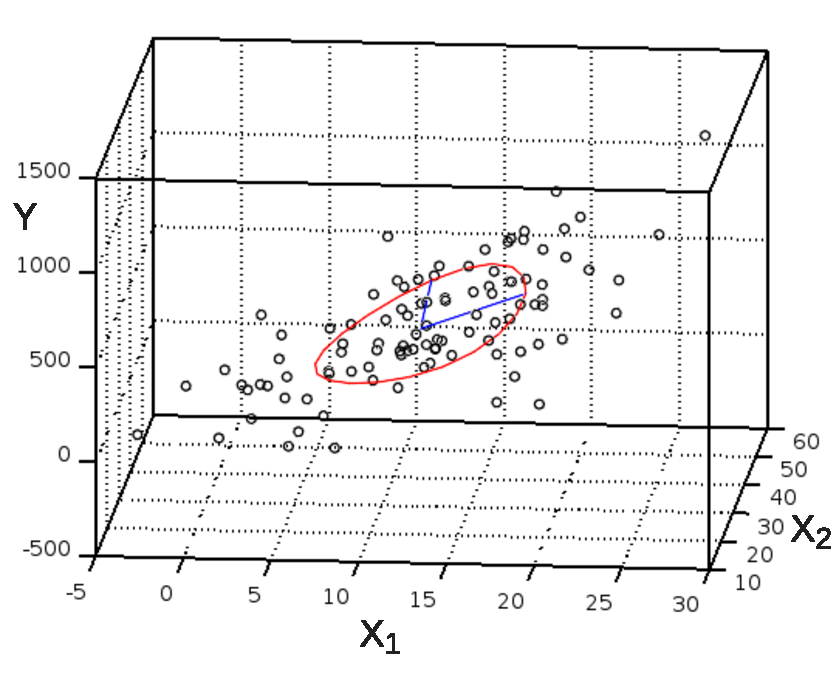
\includegraphics[width=100mm]{07_vorlesung/media/understand_fehlerfort_1.pdf}
\caption{\label{FortpfElliptisch} Eine anschauliche Deutung für die pythagoräische
Addition der Standardabweichungen liefert die Betrachtung der mit roter Kurve dargestellten
Ellipse. Die blauen Geraden repräsentieren die Abstände vom Mittelpunkt als Halbmesser
der Ellipse, die aus den Standardabweichungen jeweils von $X_1$ und $X_2$ berechnet wurden.}
\end{center}
\end{figure}
Da die beiden Größen $X_1$ und $X_2$ zwei unabhängige Dimensionen repräsentieren, werden
ihre Standardabweichungen nach dem Satz des Pythagoras addiert, eine Veranschaulichung dieses
Sachverhalts zeigt Abb.~\ref{FortpfElliptisch}. Da die Größen über die Modellgleichung
miteinander verknüpft sind und die gesuchte Standardabweichung die Dimension der Größe $Y$
trägt, müssen die Standardabweichungen der Größen $X_1$ und $X_2$ mit den entsprechenden
Sensitivitäten verknüpft werden, so dass
\begin{equation}
s_y^2 \; = \; (c_1 \, s_1)^2 \; + \; (c_2 \, s_2)^2 .
\end{equation}
Diese Varianz $s_y^2$ ist also wieder eine \textsl{kombinierte Varianz} und deren Wurzel
$s_y$ eine \textsl{kombinierte Standardabweichung}.

Für den allgemeinen Fall mit einer Linearsierung durch die Taylorreihenentwicklung
Gl.~(\ref{univarTaylorLin}) stellen die partiellen Ableitungen, also der Gradient, an
der Stelle der Schätzer der direkten Größen die Sensitivitäten 
$c_i = \left. \frac{\partial f}{\partial X_i} \right|_{\bar{\mathbf{x}}}$. Sie drücken aus,
wie stark sich die indirekte Größe $Y$ gemäß der Steigung (Gradienten) des Kurvenverlaufs des Modells 
ändert, wenn es kleine Änderungen der direkten Größen gibt. Mit anderen Worten besagt dies, wie
empfindlich die indirekte Größe auf Änderungen der direkten Größen reagiert, d.h.\ wie sensistiv
das Modell an der Position $\bar{\mathbf{x}}$ ist.

Dazu bilden wir analog zu Gl.~(\ref{KovarianzSumme}) die Varianz der gewichteten Summe
der Zufallsgrößen $\Delta X_i$
\begin{equation}
\operatorname{Var}(Y) 
= \operatorname{Var}\left(\left. f(\mathbf{X}) \right|_{\bar{\mathbf{x}}}\right) + 
\operatorname{Var}\left(\sum_{i=1}^N \left. \frac{\partial f}{\partial X_i} \right|_{\bar{\mathbf{x}}} \Delta X_i\right).
\end{equation}
Dabei sind $\left. f(\mathbf{X}) \right|_{\bar{\mathbf{x}}}$ und $c_i = \left. \frac{\partial f}{\partial X_i} \right|_{\bar{\mathbf{x}}}$ Konstanten, so dass daraus
$\operatorname{Var}\left(\left. f(\mathbf{X}) \right|_{\bar{\mathbf{x}}}\right) = 0$ und
\begin{equation}
\operatorname{Var}(Y) 
= \operatorname{Var}\left(\sum_{i=1}^N c_i \Delta X_i\right)
\end{equation}
wird, was also die Form der Gl.~(\ref{KovarianzSumme}) annimmt, so dass gilt
\begin{equation}
\operatorname {Var}\left(Y\right)
= \sum _{{i=1}}^{N} \, c_i^2 \operatorname {Var}(\Delta X_{i})+2\sum _{{i=1}}^{{N-1}}
  \sum _{{k=i+1}}^{N} \, c_i c_k \operatorname {Cov}(\Delta X_{i},\Delta X_{k})
\label{UnsicherFortpflLinearisiert}
\end{equation}
mit $\operatorname {Var}(\Delta X_{i}) = s_i^2$ für die Varianz in der Umgebung vom
Erwartungswert $\bar x_i$ und $\operatorname {Cov}(\Delta X_{i},\Delta X_{k}) = s_{i,k}$
für die Kovarianz in der Umgebung von den Erwartungswerten $\bar x_i$ und $\bar x_k$.


Zu Kapitel 5.2 im JCGM 100-Dokument des \textsl{Guide} für Messunsicherheit GUM
sei angemerkt, dass für die Sensitivitäten eine verkürzte, unmathematische Schreibweise
für die Sensitivitäten gewählt wurde, indem dort geschrieben steht $\frac{\partial f}{\partial x_i}$
anstelle von $\left. \frac{\partial f}{\partial X_i} \right|_{\bar x_1, \dots, \bar x_N}$.
Im GUM wird angemerkt dass $\frac{\partial f}{\partial x_i}$ für $\frac{\partial f}{\partial X_i}$
unter Verwendung der Schätzwerte $x_i$ zu den $X_i$.
In unserer Vorlesungsreihe sowie im GUM steht das Symbol mit dem großgeschriebenen $X_i$ für die
direkten Messgrößen. Das im GUM verwendete $x_i$ als Kleinbuchstabe steht für den Schätzwert,
was wir in der Vorlesung mit $\bar x_i$ bezeichnen. Da der Schätzwert eine Konstante ist,
kann man nach dieser natürlich nicht ableiten.


\section{Überdeckungsintervall für indirekte Messgrößen}

In Vorlesung 5 haben wir das Überdeckungsintervall behandelt, als \textsl{Credible intervall}
und als \textsl{Vertrauensintervall}. Die Intervallgrenzen des Vertrauensintervall haben wir
auch als Produkt aus einem Quantil und einer Standardabweichung repräsentiert, im Fall, dass
eine Normalverteilung zugrunde gelegt wird in der Form
\begin{equation}
\left[\bar x \, - \, z_{1-\frac{1}{2}\alpha} \, \sigma_X, 
\bar x \, + \, z_{1-\frac{1}{2}\alpha} \, \sigma_X \right]
\end{equation}
und im Fall, dass eine $t$-Verteilung zugrunde gelegt wird
\begin{equation}
\left[\bar x \, - \, t_{1-\frac{1}{2}\alpha, \nu} \, \sigma_X, 
\bar x \, + \, t_{1-\frac{1}{2}\alpha, \nu} \, \sigma_X \right]
\end{equation}
Bei dem Fall, dass eine $t$-Verteilung zugrunde gelegt wird, und zwar, wenn es um kleinere
Stichprobenumfänge geht hängt das Quantil von der Anzahl der Freiheitsgrade $\nu_i = J_i - 1$
ab, die jedoch im allgemeinen für die beiden Größen $X_i$
unterschiedlich sein kann. Es gilt also, ein gemeinsames Quantil zu finden.

Mit der bayesischen Methode, die wir zuvor betrachtet haben, konnten wir das
\textsl{Credible Interval} aus der kumulierten Posterior gewinnen. Bei dem
zuvor erörterten Beispiel Gl.~(\ref{BeispielProdukt2Gr}) $Y = X_1 X_2$ haben wir statt
der einen Likelihood drei Verteilungsdichten:
Für jede Größe $X_i$ haben wir je eine Likelihood
\begin{equation}
p_{\mathrm{L},i}(\{X_{i,1}, \dots, X_{i,J}\} | X_i, s_i) \; = \;
\prod\limits_{j=1}^J \frac{1}{\sqrt{2 \pi} \, s_i}
 e^{- \frac{1}{2} \, \left( \frac{X_{i,j} - X_i}{s_i} \right)^2 }  \; = \;
l(X_i, s_i | \{X_{i,1}, \dots, X_{i,J}\})
\end{equation}
was zwei Verteilungen liefert, und als dritte Verteilung noch
\begin{equation}
p_\mathrm{L,y}( X_1, X_2 | Y, s) \; = \;
\frac{1}{\sqrt{2 \pi} \, s}
 e^{- \frac{1}{2} \, \left( \frac{Y - X_1 \, X_2}{s} \right)^2 } 
\end{equation}
wobei dann nicht nur über $s$, sondern auch über $X_1$ und $X_2$ integriert wird, um die
Posterior als Marginalverteilung, die nur noch von $Y$ abhängt, zu erhalten.

Für relativ einfache analytische Zusammenhänge, also für explizite Modelle
und für ein\-fachere implizite Modellansätze wie die lineare Regression, ist
es nicht erforderlich die numerisch aufwendigere
kolmogoroffschen Wahrscheinlichkeitsrechnung (Bildung
der Produkte der Verteilungen) anzuwenden.
Für explizite linearisierbare Modelle 
$$
Y = f(\mathbf{X}) \qquad \mathbf{Y} = \vec f(\mathbf{X})
$$
mit $\vec f = (f_1,\dots,f_l, \dots, f_M)^\mathsf{T}$ ist das 
Fortpflanzungsgesetz gemäß Gl.~(\ref{UnsichFortpfl2}) wie folgt
\begin{equation}
u^2(Y_l) = \sum\limits_{i=1}^{N} \, \left( \left. \frac{\partial f_l(\mathbf{X})}{\partial X_i}\right|_{\bar{\mathbf{x}}} \right)^2 \, u^2(X_i) \;  + \; 
2 \, \sum\limits_{i=1}^{{N-1}}
 \sum\limits_{k=i+1}^{N} \, \left. \frac{\partial f_l(\mathbf{X})}{\partial X_i}\right|_{\bar{\mathbf{x}}} \,
 \left. \frac{\partial f_l(\mathbf{X})}{\partial X_k}\right|_{\bar{\mathbf{x}}}  \; \rho_{i,k} \, u(X_i) \, u(X_k)
\end{equation}
verwendbar. Für die lineare Regression 
$$
Y_\mathrm{Regr} = \sum_{l=1}^M \theta_i X_l
$$
die bzgl.\ der indirekten Messgrößen $\theta_l = Y_l$ ein implizites Modell ist, gilt
für die Unsicherheitsfortpflanzung Gl.~(87) mit Gl.~(88) aus Vorlesung 2.
Mit einer Stichprobe mit Tupeln $(Y_{\mathrm{Regr},j}, X_{1,j},\dots,X_{M,j})$ und mit
$\boldsymbol Y_{\mathrm{Regr}} = (Y_{\mathrm{Regr},1},\dots,Y_{\mathrm{Regr},J})^{\mathsf{T}}$
und der Regressormatrix $\boldsymbol X = (X_{l,j})$ liefert das Fortpflanzungsgesetz die
Kovarianz der Modellparameter
\begin{equation}
\operatorname{Cov}(\boldsymbol \theta) \; = \; \left(\boldsymbol X^\mathsf{T} \, \boldsymbol X\right)^{-1} \, \operatorname{Var}(\boldsymbol \varepsilon)
\end{equation}
mit $J$ für den Stichprobenumfang und $M$ für die Anzahl der Modellparameter und mit
\begin{equation}
\operatorname{Var}(\boldsymbol \varepsilon) \; = \; 
	\frac{1}{J-M}\left(\boldsymbol Y \; - \; \boldsymbol X \, \hat{\boldsymbol \theta}\right)^\mathsf{T}
\left(\boldsymbol Y \; - \; \boldsymbol X \, \hat{\boldsymbol \theta}\right)
\end{equation}
Die Hauptdiagonale der Kovarianz der Modellparameter enthält die Varianzen
$$
\sigma_{\theta_l}^2 = u^2(\theta_l\equiv Y_l)
$$
der jeweiligen Modellparameter.

Für die Ermittlung des Überdeckungsintervalls $[y_l-U(Y_l), y_l+U_l]$ wird ein entsprechender
Erweiterungsfaktor $k$ für $U(Y_l) = k \, u(Y_l)$ gebraucht. Wird als Erweiterungsfaktor das
Quantil der $t$-Verteilung eingesetzt, so wird eine \textsl{effektive Anzahl
von Freiheitsgraden} $\nu_\mathrm{eff}$ approximiert.
In Abschnitt G.4 des Dokuments JCGM 100 GUM:2008 wird auf die Berechnungsmethode
für $\nu_\mathrm{eff}$ von Satterthwaite aus dem Jahr 1941 \cite{Sat41} zurückgegriffen.

Satterthwaite betrachtet die Varianz $\operatorname{Var}(s_i^2)$
der Varianz $s_i^2$. Die $s_i^2$ sind unabhängige
Zufallsgrößen, also als Größen zu betrachten, die unkorreliert sind, so dass
\begin{equation}
\operatorname{Var}(s_y^2) \; = \;  \operatorname{Var}\left( c_1^2 s_1^2 \right)
 \; + \; \operatorname{Var}\left( c_2^2 s_2^2 \right)
\label{VarianzvarianzSumme}
\end{equation}
gilt.
Die empirischen Varianzen $s_1^2$ und $s_2^2$ der Größen $X_1$ und $X_2$ sind $\chi^2$-verteilt,
d.h.\ für die normierte Größe gilt
\begin{equation}
Q_i \; = \; \nu_i \, \left(\frac{s_i}{\sigma_i}\right)^2 \, \sim \; \chi^2(\nu_i) .
\end{equation}
Der Erwartungswert für $Q_i$ ist
\begin{equation}
\operatorname{E}(Q_i) \; = \; \int_0^\infty \; Q \; p_{\chi^2}(Q) \; \operatorname{d}Q \; = \; \nu_i.
\label{ErwartungswertQ}
\end{equation}
Die Varianz $\operatorname{Var}(Q_i)$ ist
\begin{equation}
\operatorname{Var}(Q_i) \; = \; \int_0^\infty \; (Q - \nu_i)^2 \; p_{\chi^2}(Q) \; \operatorname{d}Q \; = \; 2 \nu_i.
\label{VarianzQ}
\end{equation}
Die Herleitungen zu den beiden Gln.~(\ref{ErwartungswertQ}) und (\ref{VarianzQ})
befinden sich in Anhang \ref{ErwaChi2}.

Ferner gilt allgemein für die Varianz einer Zufallszahl $R$
multipliziert mit einem konstanten Faktor $a$
\begin{equation}
\arraycolsep=2.4pt\def\arraystretch{2}
\begin{array}{ll}
\operatorname{Var}(a R) & = \; \int\limits_0^\infty \, (a R - \operatorname{E}(a R))^2  \, p(R)  \, \operatorname{d}R \\
 & = \int\limits_0^\infty \, a^2 \, (R - \operatorname{E}(R))^2  \, p(R)  \, \operatorname{d}R\\
 & = a^2 \, \int\limits_0^\infty \, (R - \operatorname{E}(R))^2  \, p(R)  \, \operatorname{d}R\\
 & = a^2 \, \operatorname{Var}(R)
\end{array}
\end{equation}
so dass
\begin{equation}
\operatorname{Var}(Q_i) \; = \; \operatorname{Var}\left(\nu_i \, \left(\frac{s_i}{\sigma_i}\right)^2\right)
 \; = \; \left(\frac{\nu_i}{\sigma_i^2}\right)^2 \, \operatorname{Var}(s_i^2)
\end{equation}
mit Gl.~(\ref{VarianzQ}) zu
\begin{equation}
2 \nu_i \; = \; \left(\frac{\nu_i}{\sigma_i^2}\right)^2 \, \operatorname{Var}(s_i^2)
\end{equation}
wird. Das heißt
\begin{equation}
2 \nu_i \; = \; \frac{\nu_i^2}{\sigma_i^4} \, \operatorname{Var}(s_i^2)
\end{equation}
%und
%\begin{equation}
%2 \sigma_i^4  \; = \; \frac{\nu_i^2}{\nu_i} \, \operatorname{Var}(s_i)
%\end{equation}
%und
%\begin{equation}
%2 \sigma_i^4  \; = \; \nu_i \, \operatorname{Var}(s_i)
%\end{equation}
also
\begin{equation}
\operatorname{Var}(s_i^2) \; = \; \frac{2 \sigma_i^4}{\nu_i} .
\end{equation}
so dass nach Sattherthwaite aus Gl.~(\ref{VarianzvarianzSumme}) die \textsl{effektive Anzahl
der Freiheitsgrade} $\nu_\mathrm{eff}$ für die Größe $Y$, also $\nu_\mathrm{eff} = \nu_y$
abgeschätzt wird mit
$$
\frac{2 \sigma_y^4}{\nu_y} \; = \;  \frac{2 c_1^4 \sigma_1^4}{\nu_1} 
 \; + \; \frac{2 c_2^4 \sigma_2^4}{\nu_2}
$$
mit $\operatorname{Var}(s_y^2) \; = \; \frac{2 \sigma_y^4}{\nu_y}$ 
und nach Rauskürzen des Faktors 2
\begin{equation}
\frac{\sigma_y^4}{\nu_y} \; = \;  \frac{c_1^4 \sigma_1^4}{\nu_1} 
 \; + \; \frac{c_2^4 \sigma_2^4}{\nu_2}
\label{Satterthwaite}
\end{equation}
so dass
\begin{equation}
\nu_y \; = \; \frac{\sigma_y^4}{\frac{(c_1 \, \sigma_1)^4}{\nu_1} 
 \; + \; \frac{(c_2 \, \sigma_2)^4}{\nu_2}} .
\label{EffectiveDFfuer2}
\end{equation}
Wenn mit Gleichung (\ref{ErwartungswertQ}) der Erwartungswert 
von $Q$ gleich der Anzahl der Freiheitsgrade ist, also $\operatorname{E}(Q) = \nu$
für $Q = \nu \left(\frac{s}{\sigma}\right)^2$, dann ist der Erwartungswert der
Varianz $s^2$
\begin{equation}
\operatorname{E}(s^2) \; = \; \operatorname{E}(\frac{\sigma^2}{\nu} Q)
\end{equation}
und mit $\frac{\sigma^2}{\nu}$ als konstanter Faktor bezüglich der Wahrscheinlichkeitsdichte
und mit Gl.~(\ref{ErwartungswertQ}) erhalten wir
\begin{equation}
\operatorname{E}(s^2) \; = \; \frac{\sigma^2}{\nu}  \operatorname{E}(Q) \; = \; 
\frac{\sigma^2}{\nu} \nu \; = \; \sigma^2
\end{equation}
und wir setzten in Gl.~(\ref{EffectiveDFfuer2}) die Erwartungswerte
$\operatorname{E}(s_y^2)$, $\operatorname{E}(s_1^2)$ und $\operatorname{E}(s_2^2)$ ein,
deren Schätzer die empirisch ermittelten Varianzen sind.

Das $t$-Quantil wird damit für $\nu_y = \nu_\mathrm{eff}$ berechnet und das vollständige Messergebnis wie folgt
angegeben
\begin{equation}
Y \; = \; y \, \pm \, t_{1-\alpha/2,\nu_y} s_y .
\label{vollstaendigesSatterthwaite}
\end{equation}


Verallgemeinert für $N$ direkte Größen ist dies
\begin{equation}
\nu_\mathrm{eff} \; = \; \frac{\sigma_y^4}{\sum\limits_{i=1}^N \frac{(c_i \, \sigma_i)^4}{\nu_i}} .
\label{EffectiveDFviele}
\end{equation}


Aufgrund der Verallgemeinerung, dass \textsl{Überdeckungsintervalle} sowohl
klassisch ermittelte Vertrauensintervalle als auch bayesisch ermittelte
\textsl{Credible Intervals} sein können,
werden die zu einer gewissen Wahrscheinlichkeit $1-\alpha$ gehörenden Faktoren
\textsl{Erweiterungsfaktor} genannt. Sei  $[z_\mathrm{min}, z_\mathrm{max}]$
das \textsl{Credible Interval}
einer Größe $Y$ mit Posterior $p(Y |\dots)$ deren Erwartungswert
\begin{equation}
\bar Y \; = \; \int\limits_{-\infty}^\infty \, Y \, p(Y |\dots) \, \operatorname{d}Y
\end{equation}
und deren Varianz
\begin{equation}
\operatorname{Var}(Y) \; = \; \int\limits_{-\infty}^\infty \, (Y - \bar Y)^2 \, p(Y |\dots) \, \operatorname{d}Y
\end{equation}
ist, so ist der \textsl{Erweiterungsfaktor} $k$ für symmetrische Verteilungen mit
$z_\mathrm{max} - \bar Y = \bar Y - z_\mathrm{min}$
\begin{equation}
k \; = \; \frac{z_\mathrm{max} - \bar Y}{\sqrt{\operatorname{Var}(Y)}}
\end{equation}
was für klassische Berechnungsverfahren dem 
t-Quantil $t_{1-\alpha/2,\nu_\mathrm{eff}}$ entspricht
\begin{equation}
k \; = \; t_{1-\alpha/2,\nu_\mathrm{eff}} .
\end{equation}
Für symmetrische Verteilungen ist die halbe Breite des Überdeckungsintervalls
gleich der \textsl{erweiterten Messunsicherheit} der Größe $Y$. Die
\textsl{erweiterte Messunsicherheit} kann das Produkt aus
Erweiterungsfaktor und empirischer Standardabweichung sein.

Während mit \textsl{kleinem} Buchstaben $u$ die Standardabweichungen bezeichnet werden,
werden mit \textsl{großem} Buchstaben $U$ die erweiterten Unsicherheiten geschreiben, die das Produkt aus
dem Erweiterungsfaktor $k$, der in der klassischen Statistik das $t$-Quantil ist, und der Unsicherheit $u$ ist,
sind.

\section{Vergleich der klassischen mit der bayesischen Methode}

Als nächstes wollen wir zeigen, dass für die \glqq gutmütigen\grqq ~Fälle, für die das
Gesetz der Mess\-un\-sicher\-heits\-fort\-pflanz\-ung anwendbar ist, die Berechnung des vollständigen
Ergebnisses unter Verwendung der Methode der bayesischen Statistik im wesentlichen dasselbe
Resultat liefert wie unter Verwendung des Fort\-pflanz\-ungs\-gesetzes.

Wir betrachten ein Beispiel, bei dem irgendeine physikalische Größe zu messen ist.
Dabei werde ein Gerät bzw.\ Sensor verwendet, dessen Funktionsprinzip auf einem
physikalischen Effekt beruht und dadurch die Größe so erfasst,
dass als direkte Messgröße eine Spannung in Volt angezeigt wird. Dies kann beispielsweise
die Messung einer Temperatur sein, in der das Phänomen, dass sich ein elektrischer
Widerstand proportional zur Tempertur verändert und die Widerstandsänderung über die
Änderung der elektrischen Spannung, die über dem Widerstand abfällt, bestimmt wird.
Dies kann beispielsweise eine Stufenhöhe sein, die mit Hilfe eines induktiven Wegaufnehmers
gemessen wird, der auf dem Phänomen beruht, dass sich die Induktivität einer Spule in Abhängigkeit
von der  Position ihres Ferritkerns verändert. Es sind viele Beispiel denkbar. Sensoren
sind oft so konzipiert, dass sie ein physikalisches Phänomen nutzen und zur elektronischen
Erfassung der zu messenden Größe als direkte Größe ein Messignal in Form einer elektrischen
Spannung liefern.

Wir wollen im folgenden ganz allgemein die indirekte Messgröße mit $Y$
bezeichnen und uns auf keine physikalische Einheit festlegen, sondern diese allgemein nur
\glqq Einheit\grqq ~nennen. Das Modell, das wir betrachten, ist wie folgt: Das rohe Messsignal,
das als Spannung $U$ bzw.\ direkte Größe $X_\mathrm{M}$ vorliegt, ist über
einen Kalibrierfaktor $K$ bzw.\ eine direkte Größe $X_\mathrm{K}$
in die physikalische Einheit der indirekten physikalischen Größe $Y$ umzurechnen. 
Der Index M steht hier für Messung und der Index K für Kalibrierfaktor.

Die indirekte Größe $Y$ habe irgendeine physikalische Einheit $\mathrm{E}$
\begin{equation}
Y \; = \; f(X_\mathrm{K}, X_\mathrm{M})  \; = \; X_\mathrm{K} \, X_\mathrm{M}
\end{equation}
und die beiden direkten Größen $X_\mathrm{M}$ und $X_\mathrm{K}$ 
sollen die Einheiten Volt $\mathrm{V}$ und $\frac{\mathrm{E}}{\mathrm{V}}$
haben.

%In der siebten Vorlesung hatten wir anhand dieses Beispiels die
%Wahrscheinlichkeitsdichteverteilungen, engl.\ (\textsl{Probability Density Function}, kurz PDF)
%betrachtet und verschiedene Vorstellungen darüber, wie sich die Unsicherheit der indirekten
%Messgröße zusammensetzt, verglichen. Die eine Sichtweise war, dass wir die Unsicherheit des
%Sensors $s_\mathrm{S}$ aus vorherigen Untersuchungen des Gerätes genau kennen und dass diese
%deutlich kleiner sei als die Streuung der aktuell vorliegenden Beobachtungen, also dass die
%Streuung $s_\mathrm{M}$ von der Streuung des Gegenstands der Messung dominiert werde. Die andere
%Sichtweise war, dass wir nichts über die Unsicherheit des Sensors wissen, also kein Wert zu
%$s_\mathrm{S}$ vorliege und nur die empirische Streuung $s_\mathrm{M}$ aus den
%Beobachtungen ermittelt wird. Die dem Sensor intrinsische Unsicherheit bleibt im zweiten Fall
%unerkannt.

Die Stichprobe der Beobachtungen zum rohen Messignal habe einen recht kleinen
Umfang $J_\mathrm{M} = 9$:

\begin{tabular}{l|c|c|c|c|c|c|c|c|c}
\hline
$X_\mathrm{M} / \mathrm{V}$ &  479.58 &  526.47 &  516.77 &  522.01 &  506.61 &  497.99 &  481.71 &  484.90 &  491.41\\
\hline
\end{tabular}

Als vollständiges Messergebnis zum Kalibrierfaktor $X_\mathrm{K}$ liegen uns folgende Angaben vor
$$
X_\mathrm{K} \; = \; (K_0 \, \pm \, U_\mathrm{K}) \, \frac{\mathrm{E}}{\mathrm{V}}
 \; = \; (0.0925 \, \pm \, 0.0180) \, \frac{\mathrm{E}}{\mathrm{V}}
 \qquad \mathrm{mit} \qquad k = 2 \quad \mathrm{und} \quad \nu_\mathrm{K} = 45
$$
Der Erweiterungsfaktor $k = 2$ ist der gerundete Wert für das 
t-Quantil für $95 \, \%$ Vertrauensniveau $\nu_\mathrm{K} = 45$ Freiheitsgrade.
Der genauere Wert wäre $k = 2.0141$, die Rundung ist hier zulässig.

Wir beleuchten den Fall, dass wir die dem Sensor intrinsische Unsicherheit nicht kennen, aber
davon ausgehen, dass die Unsicherheit $\sigma_\mathrm{winzig}$ aufgrund der
Modellapproximation für die Sensorik, hier also u.a.\ dass vorausgesetzt wird,
dass der Sensor linear ist, wesentlich kleiner ist als die Streuung der Messvorgänge beim
Erfassen der Rohdaten und der Sensorkalibrierung:
\begin{equation}
\arraycolsep=2.0pt\def\arraystretch{2.0}
\begin{array}{l}
p(Y, X_\mathrm{K}, X_\mathrm{M} | (X_{\mathrm{M},1}, \dots, X_{\mathrm{M},J}), K_0, s_\mathrm{K}) \propto \\
e^{-\frac{1}{2} \left(\frac{ Y \; - \; X_\mathrm{K} \, X_\mathrm{M}}{\sigma_\mathrm{winzig}} \right)^2}
\;  e^{-\frac{1}{2} \left(\frac{X_\mathrm{K} - K_0}{s_\mathrm{K}} \right)^2} \; \prod\limits_{j=1}^J  \,
e^{-\frac{1}{2} \left(\frac{ X_\mathrm{M} - X_{\mathrm{M},j} }{s_\mathrm{M}} \right)^2}
\end{array}
\label{PosteriorFall3}
\end{equation}
mit $\sigma_\mathrm{winzig} \; = \; 0.003 \cdot s_\mathrm{KM}$, mit $s_\mathrm{KM}  \; = \; K_0 \,
s_\mathrm{M}$ und mit $s_\mathrm{K} = \frac{U_\mathrm{K}}{2} = 0.0090$.
Wir verwenden zur Berechnung der Likelihood die empirische Standardabweichung der Daten zu $X_M$:
$$
\bar x_\mathrm{M} \, = \, \frac{1}{9} \sum_{j=1}^9 X_{\mathrm{M},j} \, = \, 500.83 \, \mathrm{V}
$$
und
$$
s_\mathrm{M} \, = \, \sqrt{ \frac{1}{\nu_\mathrm{M}} \sum_{j=1}^9 (X_{\mathrm{M},j} - \bar x_\mathrm{M})^2 }
 \, = \, 17.8927 \, \mathrm{V} \, \approx \,  17.89 \, \mathrm{V} 
$$
mit $\nu_\mathrm{M} = 8$ Freiheitsgraden,
damit also  
$K_0 \, s_\mathrm{M} \, = \, s_\mathrm{KM} \, = \, 1.655 \, \mathrm{E}$ und entsprechend für $\sigma_\mathrm{winzig} \, = \, 0.00497$.
Da die Stichprobenwerte
der Größe $X_\mathrm{M}$ in der Tabelle mit 2 Nachkommastellen angegeben werden, wird das Ergebnis
auch auf 2 Stellen gerundet.


Wir bestimmen den Schätzer und das Überdeckungsintervall im folgenden zum einen aus der
Unsicherheitsfortpflanzung gemäß (\ref{UnsichFortpfl2})
und zum anderen aus der Marginalverteilung zu Gl.~(\ref{PosteriorFall3}):
\begin{equation}
\arraycolsep=2.0pt\def\arraystretch{2.0}
\begin{array}{l}
p(Y | (X_{\mathrm{M},1}, \dots, X_{\mathrm{M},J}), K_0, s_\mathrm{K}) \; = \;\\
\frac{\int\limits_{-\infty}^\infty \int\limits_{-\infty}^\infty \,
e^{-\frac{1}{2} \left(\frac{ Y \; - \; X_\mathrm{K} \, X_\mathrm{M}}{\sigma_\mathrm{winzig}} \right)^2}
\;  e^{-\frac{1}{2} \left(\frac{X_\mathrm{K} - K_0}{s_\mathrm{K}} \right)^2} \; \prod\limits_{j=1}^J \,
 e^{-\frac{1}{2} \left(\frac{ X_\mathrm{M} - X_{\mathrm{M},j} }{s_\mathrm{M}} \right)^2} \,
\operatorname{d}X_\mathrm{M} \, \operatorname{d}X_\mathrm{K} }
{\int\limits_{-\infty}^\infty  \int\limits_{-\infty}^\infty \int\limits_{-\infty}^\infty \,
e^{-\frac{1}{2} \left(\frac{ Y \; - \; X_\mathrm{K} \, X_\mathrm{M}}{\sigma_\mathrm{winzig}} \right)^2}
\; e^{-\frac{1}{2} \left(\frac{X_\mathrm{K} - K_0}{s_\mathrm{K}} \right)^2} \;\prod\limits_{j=1}^J \,
 e^{-\frac{1}{2} \left(\frac{ X_\mathrm{M} - X_{\mathrm{M},j} }{s_\mathrm{M}} \right)^2} \,
\operatorname{d}X_\mathrm{M} \, \operatorname{d}X_\mathrm{K} \, \operatorname{d}Y}
\end{array}
\label{marginalPosteriorFall2}
\end{equation}
Wir erhalten den Schätzwert $\bar y$ aus
\begin{equation}
\bar y \; = \; \int\limits_{-\infty}^\infty \, Y \, 
p(Y | (X_{\mathrm{M},1}, \dots, X_{\mathrm{M},J}), K_0, s_\mathrm{K}) \, \operatorname{d}Y
\label{ErwartungswertY}
\end{equation}
und für die Bestimmung der Intervallgrenzen $y_1, y_2$ für das Überdeckungsintervall
berechnen wir die kumulierte Verteilung
\begin{equation}
P(Y) \; = \;  \int\limits_{-\infty}^Y \, 
p(Y^\prime | (X_{\mathrm{M},1}, \dots, X_{\mathrm{M},J}), K_0, s_\mathrm{K}) \, \operatorname{d}Y^\prime
\label{cdfBeispiel}
\end{equation}
und dann für $95 \%$ Wahrscheinlichkeit
\begin{equation}
P(y_1) \, = \, 0.025 \; \Leftrightarrow \; y_1 \, = \, P^{-1}(0.025) 
\qquad \mathrm{und} \qquad P(y_2) \, = \, 0.975 \;
\Leftrightarrow \;  y_2 \, = \, P^{-1}(0.975) .
\end{equation}


Durch numerische Integration der Gl.~(\ref{ErwartungswertY}) erhalten wir
$$
\bar y \; = \; 46.278 \, \mathrm{E}
$$
und für das \textsl{Credible Interval} durch numerische Integration von Gl.~(\ref{cdfBeispiel})
$$
[36.855 \, \mathrm{E}, 56.185 \, \mathrm{E}] \; = \; [\bar y - 9.423, \bar y + 9.907] \, \mathrm{E}
$$
und vergleichen dieses Ergebnis mit dem Ergebnis, das wir auf dem klassischen Wege erhalten. Zunächst
berechnen wir das Produkt der beiden Werte $\bar x_\mathrm{M} = 500.83 \, \mathrm{V}$ und
$K_0 = 0.0925 \, \frac{\mathrm{E}}{\mathrm{V}}$. Wir erhalten mit
$$
\bar y \, = \, K_0 \, \bar x_\mathrm{M} \; = \; 46.327 \, \mathrm{E}
$$
einen Schätzwert für $Y$, der um einen Wert von $0.049 \, \mathrm{E}$ also um 1 Promille von dem aus der
bayesischen Berechnung differiert.

In Anhang \ref{AnhangBayesBeispiel} befindet sich das Gnu-Octave/Matlab-Skript, mit dem die Berechnungen zu diesem
Beispiel durchgeführt wurden,.

Als nächstes vergleichen wir das \textsl{Credible Interval} mit dem
Vertrauensintervall. Dazu bestimmen wir die Unsicherheit mit
dem Fortpflanzungsgesetz für unkorrelierte direkte Messgrößen.

\begin{figure}
\begin{center}
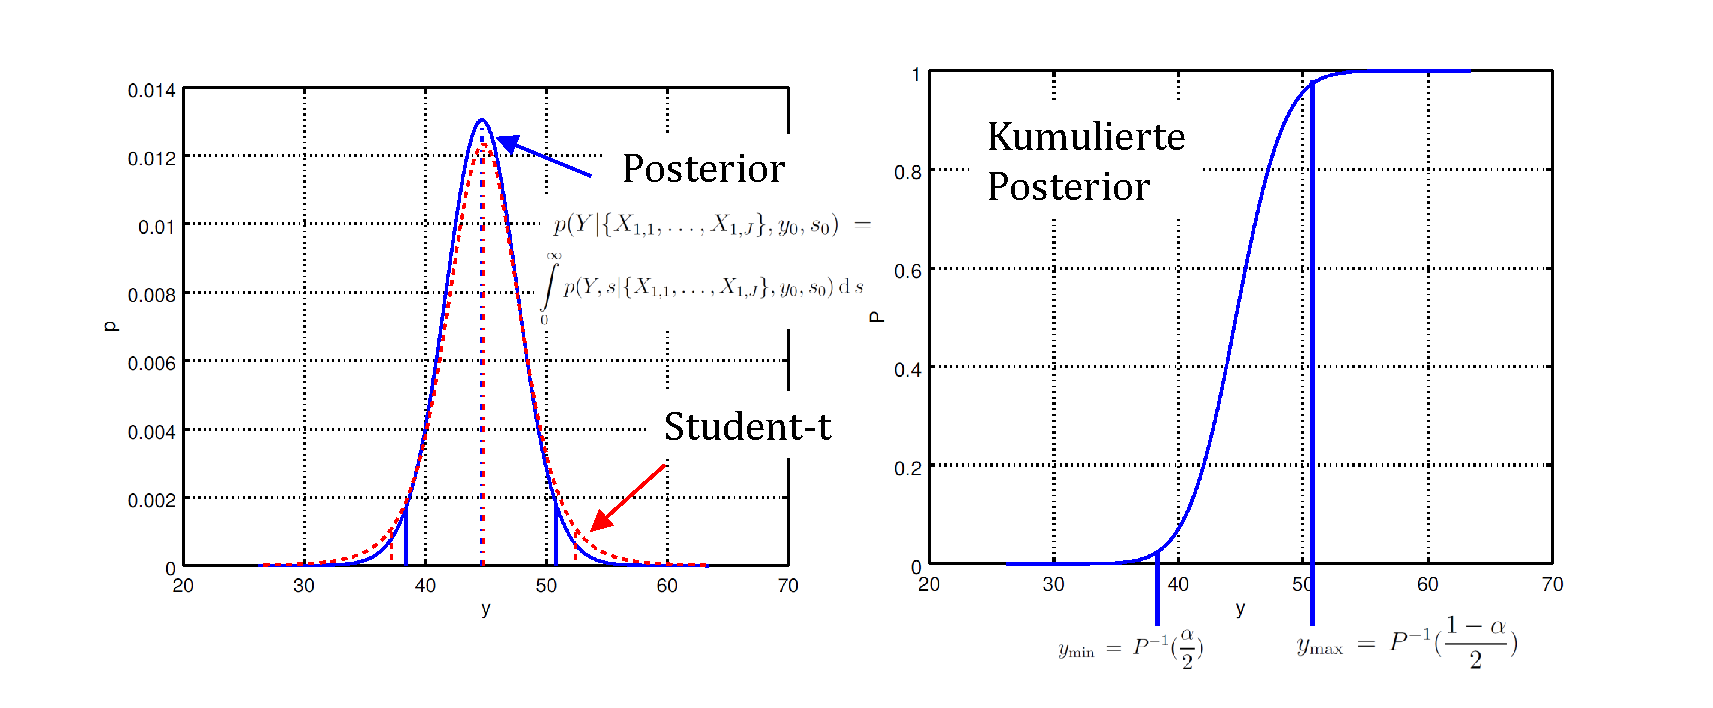
\includegraphics[width=160mm]{07_vorlesung/media/Ueberdeckungsintervall_0.pdf}
\caption{\label{VergleichsBeispiel}Wahrscheinlichkeitsdichtefunktionen und kumulierte Posterior
für die Bestimmung des Überdeckungsintervalls einer indirekten Messgröße}
\end{center}
\end{figure}
Wir berechnen für $\rho_{\mathrm{M}, \mathrm{K}} = 0$
$$
u^2(Y) \; = \;
\left(\frac{\partial}{\partial X_\mathrm{M}} X_\mathrm{M} X_\mathrm{K} 
\right)^2_{\bar x_\mathrm{M}, K_0} \, s_\mathrm{M}^2 \; + \;
\left(\frac{\partial}{\partial X_\mathrm{K}} X_\mathrm{M} X_\mathrm{K} 
\right)^2_{\bar x_\mathrm{M}, K_0} \, s_\mathrm{K}^2
$$
d.h.
$$
u(Y) \; = \;
\sqrt{ K_0^2 \, s_\mathrm{M}^2 \; + \; \bar x_\mathrm{M}^2 \, s_\mathrm{K}^2 }
\; = \; 4.802 \, \mathrm{E} .
$$
Die Anzahl der Freiheitsgrade berechnen wir gemäß der Satterthwaite'schen Gleichung
(\ref{EffectiveDFviele}), also
$$
\frac{u(Y)^4}{\nu_y} \; = \; \frac{K_0^4 \, s_\mathrm{M}^4}{\nu_\mathrm{M}} \; + \;
\frac{\bar x_\mathrm{M}^4 \, s_\mathrm{K}^4}{\nu_\mathrm{K}}
$$
d.h.\ mit $\nu_\mathrm{K} = 45$, $\nu_\mathrm{M} = 8$ und mit
$K_0 = 0.0925 \, \frac{\mathrm{E}}{\mathrm{V}}$, $s_\mathrm{K}=0.009 \, \frac{\mathrm{E}}{\mathrm{V}}$,
$\bar x_\mathrm{M} = 500.83 \, \mathrm{V}$, $s_\mathrm{M} = 17.89 \, \mathrm{V}$
$$
\nu_y \; = \; u(Y)^4 \, \left( \frac{K_0^4 \, s_\mathrm{M}^4}{\nu_\mathrm{M}} \; + \;
\frac{\bar x_\mathrm{M}^4 \, s_\mathrm{K}^4}{\nu_\mathrm{K}} \right)^{-1} \; = \;
52.58 \; \approx \; 52
$$
Die Anzahl der Freiheitsgrade kann auf ganzzahlige Werte abgerundet werden, das heißt die Nachkommastellen
 unterdrückt werden, siehe GUM JCGM 100:2008, Seite 73:
\begin{quote}
NOTE 1 If the value of $\nu_\mathrm{eff}$ obtained from Equation (G.2b) is not an integer,
which will usually be the case in practice, the corresponding value of $t_\mathrm{p}$ may be found
from Table G.2 by interpolation or by truncating $\nu_\mathrm{eff}$ to the next lower integer.
\end{quote}
\begin{verbatim}
>> tinv(0.975,52)
ans =  2.0066
>> tinv(0.975,52.58)
ans =  2.0061
\end{verbatim}
Wir verwenden für das t-Quantil (den Erweiterungsfaktor) den Wert $k = 2.006$, in der Praxis
nimmt man dann auch einfach $k = 2$.
Gemäß GUM kann die Formel für die effektive Anzahl von Freiheitsgraden also auch wie folgt
geschrieben werden
\begin{equation}
\nu_y \; = \;  \lfloor u(Y)^4 \, \left( \sum\limits_{i=1}^N \, \frac{ (c_i \, s_i)^4}{\nu_i}  \right)^{-1} \rfloor 
\label{SatterthwaiteFloor}
\end{equation}
wobei die beiden Symbole $\lfloor r \rfloor$ um die Variable $r$ geschrieben heißen, dass
die Nachkommastellen von $r$ abzuschneiden sind, was in vielen Programmiersprachen mit der
Funktion \texttt{floor} erfolgt.

Das Vertrauensintervall wird damit schließlich
$$
[36.691 \, \mathrm{E}, 55.962 \, \mathrm{E}]
$$
und das vollständige Messergebnis
$$
Y \; = \; (46.327 \pm 9.635) \, \mathrm{E} .
$$
Der Wert für die erweiterte Unsicherheit $U = 9.635 \, \mathrm{E}$ entspricht also in etwa
dem Mittelwert aus den Berechnungen aus dem bayesischen Ansatz $\frac{1}{2} (9.423 + 9.907) =  9.665$.
Abb.~\ref{VergleichsBeispiel} zeigt das Prinzip anhand eines ähnlichen Beispiels, die eingezeichneten Werte
liegen weiter auseinander, um die Intervalle besser einzeichnen zu können.

%Bevor sich die Methoden der Kolmogoroffschen Wahrscheinlichkeitsrechnung, gemeinsame Verteilungen (\textsl{joined
%probability density distributions}) und entsprechende Margnalverteilungen zu berechnen, in der Metrologie
%(JCGM-Dokumente 101 und 102) durchgesetzt hatten, teils auch wegen der höheren Anforderungen an die Rechenleistung,
%hat man sich damit beholfen, in die Unsicherheitsfortpflanzung gemäß Gl.~(\ref{UnsicherFortpflLinearisiert}) anstelle
%von Varianzen normalverteilter oder $t$-verteilter Größen für einzelne Summanden auch

%Zu dem Kalibrierfaktor hatten wir die Anzahl der Freiheitsgrade als Information vorliegen.
%Oftmals liegen {\`a}-priori Informationen zu direkten Größen vor, ohne dass die Anzahl der
%Freiheitsgrade bekannt ist und auch ohne dass genauere Informationen zur Art der Verteilung vorliegen.
%Wie wir in der letzten Vorlesung schon gelernt haben, wird in einigen Fällen angenommen, dass
%die Verteilung sogar eine Rechteckverteilung ist, das heißt dass die Werte gleichverteilt über ein
%Intervall sind. Wir haben in dem Zusammenhang den Begriff der \textbf{Ermittlungsmethode Typ B der Messunsicherheit}
%eingeführt. 

Für Größen, deren Messunsicherheit nicht unmittelbar aus vorliegenden
Stichproben gewonnen wurde, so dass Stichprobenumfang und Verteilungen nicht ermittelt
werden können, wird auf Basis heuristischer Vorstellungen eine Abschätzung der Anzahl der Freiheitsgrade
vorgenommen.

In Fällen, bei denen es um Präzisionsmessungen geht, kann vielfach angenommen werden,
dass die Anzahl der Freiheitsgrade gegen unendlich konvergiert.
\begin{equation}
\lim\limits_{\nu_i \rightarrow \infty} \, \left\{ \frac{ (c_i \, s_i)^4}{\nu_i} \right\} \; = \; 0
\end{equation}
Dies ist in Anhang G, Absatz G.4.3 des GUM JCGM 100:2008 nachzulesen. Lässt sich nicht
voraussetzen, dass die Anzahl der Freiheitsgrade sehr, sehr groß ist, so wird diese
abgeschätzt. Wie bei der Satterthwaite-Gleichung selbst, wird auch hier die Varianz der Varianz
%, siehe Anhang E, Absatz E.4.2
%\begin{equation}
%\operatorname{Var}(\bar s_i) \; \approx \; \frac{1}{2 \nu} \bar \sigma_i^2 ,
%\end{equation}
%wobei $\bar s_i$ die \textbf{empirische} Standardabweichung des Mittelwertes einer Größe $X_i$
%ist und $\bar \sigma_i = Var(X_i)$ die Standardabweichung dieser Größe ist, GUM Gl (E.7).
%Die Herleitung dieses Zusammenhangs ergibt sich aus der $\chi^2$-Verteilung, siehe Vorlesung 4 vom
%13.~November, Gln (33) bis (38) und 5.~Anhang \glqq Erwartungswerte zur $\chi^2$-Verteilung\grqq :
%$\operatorname{Var}(Q) = 2 \nu$ mit
%$Q = \nu \left(\frac{s}{\sigma}\right)^2$, so dass für die Standardabweichung der Einzelwerte gilt
\begin{equation}
\nu \; \sim \; \frac{\sigma_i^2}{\operatorname{Var}(s_i)}
\label{DFvsVariance}
\end{equation}
betrachtet, siehe Vorl 4, Gl (38) und GUM Anhang G, Absatz G.4.2.
Die Zuverlässigkeit der als {\`a}-priori Information mitgeteilten Unsicherheit muss
abgeschätzt werden mit einem bestimmten Prozentsatz
$(1 - \alpha) \cdot 100 \, \%$. Daraus wird heuristisch in Anlehnung an den
Zusammenhang (\ref{DFvsVariance}) die Anzahl der Freiheitsgrade abgeschätzt mit
\begin{equation}
\nu \; \approx \; \frac{1}{2 \alpha^2} .
\end{equation}
Der Quotient $\alpha$ wird als relative Unsicherheit $\frac{\Delta u}{u}$ der Unsicherheit $u$
interpretiert.

Nachdem wir gesehen haben, wie handlich die Berechnungen mit der klassischen Fortpflanzung
gegenüber den Methoden mit den Wahrscheinlichkeitsdichteverteilungen ist,
fragt man sich natürlich, weshalb wir den numerischen Aufwand mit dem Berechnen der
Integrale der Wahrscheinlichkeitsdichteverteilungen betreiben.
Für dieses kleine, handliche und anschauliche Beispiel ist dies selbstverständlich nicht
gerechtfertigt. Es dient lediglich dazu, das Grundprinzip des Verfahrens zu verdeutlichen.

Bei den Aufgaben, für die die Voraussetzungen zur Berechnung der Unsicherheit einer
indirekten Messgröße gemäß Gl.~(\ref{UnsichFortpfl2}) nicht mehr gegeben sind, werden die
Verfahren mit Berechnung von Wahrscheinlichkeitsdichteverteilungen eingesetzt.
Dies sind Verfahren die entweder auf der Multiplikation von Likelihoodverteilungen - letztlich
auf Monte-Carlo-Berechnungen gemäß dem JCGM 101-Dokument der GUM-Reihe - oder auf der
bayesischen Statistik basieren.
Die Multiplikation von Likelihoodverteilungen setzt im Gegensatz zur bayesischen Statistik eine
\textsl{scharfe} \glqq Verteilung\grqq ~für die Modellfunktion ein. Dabei wird hier mit dem Begriff
\textsl{scharfe} Verteilung eine Wahrscheinlichkeitsdichte bezeichnet, die als Normalverteilung
mit dem Grenzübergang für $\sigma_\mathrm{winzig} \rightarrow 0$ in eine Dirac'schen Deltafunktion übergeht.
Den Begriff \glqq Verteilung\grqq ~setzen wir hier in Anführungsstriche, weil
so eine Dirac'sche Deltafunktion der Grenzfall ist, bei dem die Verteilung keine Verteilung mehr ist,
weil die Werte scharf und nicht mehr verteilt sind.

Bei dem Beispiel (mit Gun-Octave/matalb-Skript in Anhang \ref{AnhangBayesBeispiel}) 
haben wir die numerischen Integrationen in
sehr schlichter Weise dadurch realisiert, dass wir die betreffenden Größen in ein Raster äquidistanter
Stützstellen diskretisiert haben und dann einfach summiert haben. Es sollte hiermit nur das Grundprinzip der
Verfahren der \textsl{kolmogoroffschen Wahrscheinlichkeitsrechnung} aufzeigen, die auch die Basis für die
Methoden der \textsl{bayesischen Statistik} bildet.

In vielen Fällen ist es aber nicht angesagt, beim numerischen Integrieren so zu verfahren.
Das nächste Kapitel soll deshalb einen kurzen
Überblick über unterschiedliche Verfahren zur numerischen Integration liefern.


\section{Aufgabe zum Selbststudium}
\label{AufgVor7}
Es sollen Abstände auf einem Werkstück mit Hilfe eines induktiven Wegaufnehmers gemessen werden.
Das Messprinzip eines induktiven Wegaufnehmers beruht darauf, dass
eine Wechselspannung ein Spulensystem im Sensor anregt.
Ein bewegliches ferro-magnetisches Teil am Sensor
beeinflusst die Induktivität in den Spulen.
Diese - in den Spulenteilen unterschiedliche - Induktivitätsveränderung wird vom
Messverstärker ausgewertet und in ein positions-proportionales Gleichspannungssignal
umgewandelt.

Um die Abstände in der physikalischen Einheit Mikrometer zu erhalten, muss mit Hilfe
eines Bezugsnormals aus dem Spannungssignal ein Weg mit der Dimension einer Länge
berechnet werden.
Es ist bekannt, dass in dem für die Messung relevanten Messbereich (Hub des Sensors)
die Abhängigkeit zwischen Spannungssignal und Auslenkung des ferro-magnetischen Kerns
linear ist.
Das Bezugsnormal ist eine Stufenhöhe.

Zu dem Bezugsnormal gibt es einen Kalibrierschein, der folgenden Höhenwert für das
Normal angibt:
\begin{equation}
d \; = \; (4.997 \pm 0.011) \; \mathrm{\mu m} \qquad \mathrm{mit} \qquad k = 2.1, \nu = 26
\label{kalBezug}
\end{equation}

Mit dem induktiven Wegaufnehmer wurden auf dem Bezugsnormal folgende Stufenhöhen in
der Dimension der elektrischen Spannung mit der Einheit Millivolt gemessen

% muB = 200; sigB = 8;
% JB = 11; xB = muB+sigB*randn(1,JB);
% printf("& %4.1f ", xB);
% xB = [201.3  187.3  196.5  200.4  193.6  174.2  197.2  185.4  194.4  202.5  205.2];
Tabelle A5.1:\\
\begin{tabular}{c||c|c|c|c|c|c|c|c|c|c|c}
\hline
$U_\mathrm{B} / \mathrm{mV}$ & 201.3 & 187.3 & 196.5 & 200.4 & 193.6 & 174.2 & 197.2 & 185.4 & 194.4 & 202.5 & 205.2\\
\hline
\end{tabular}

%Für den Abstand auf dem Werkstück wurden folgende Spannungen gemessen
%>> muW = 180; sigW = 11;
%>> JW = 7; xW = muW+sigW*randn(JW,1);
%>> printf(" %4.1f ", xW);
% 176.5  184.1  180.5  193.6  176.0  194.5  160.9 >>
%>> printf("& %4.1f ", xW);
Tabelle A5.2:\\
\begin{tabular}{c||c|c|c|c|c|c|c}
\hline
$U_\mathrm{W} / \mathrm{mV}$ & 176.5 & 184.1 & 180.5 & 193.6 & 176.0 & 194.5 & 160.9 \\
\hline
\end{tabular}

Der Zusammenhang zwischen dem Abstand auf dem Werkstück in Mikrometern $d_\mathrm{W}$,
der Stufenhöhe des Bezugsnormals gemäß Kalibrierschein $d$, dem gemessenen Spannungssignal
an der Stufenhöhe $U_\mathrm{B}$ und dem gemessenen Spannungssignal $U_\mathrm{W}$ am Werkstück
ist folgender
\begin{equation}
d_\mathrm{W} \; = \; \frac{d}{U_\mathrm{B}} \, U_\mathrm{W}
\end{equation}

Die Änderungen aufgrund der statistischen Streuung der Spannungswerte $U_\mathrm{B}$ sind
so klein, dass für die Sensitivität $c_\mathrm{B}$ von $d_\mathrm{W}$
bezüglich Änderungen von $U_\mathrm{B}$
mit dem hyperbolischen Zusammenhang $d_\mathrm{W} \sim \frac{1}{U_\mathrm{B}}$ 
die Steigung der Tangenten an die Hyperbel verwendet wird. Es wird die
Tangente verwendet, die an dem Punkt, der sich aus den Mittelwerten
ergibt, anliegt.
\begin{equation}
c_\mathrm{B} \; = \; \left. \frac{\partial}{\partial U_\mathrm{B}}
 d_\mathrm{W} \right|_{\bar U_\mathrm{B}, \bar d, \bar U_\mathrm{W}}
\end{equation}
Die Sensitivitäten $c_\mathrm{d}$ und $c_\mathrm{W}$ von $d_\mathrm{W}$
bezüglich Änderungen von $d$ und $U_\mathrm{W}$ sind aufgrund des
linearen Zusammenhangs genau
\begin{equation}
c_\mathrm{d} \; = \; \left. \frac{U_\mathrm{W}}{U_\mathrm{B}} \right|_{\bar U_\mathrm{B}, \bar U_\mathrm{W}} \qquad
c_\mathrm{W} \; = \; \left. \frac{d}{U_\mathrm{B}} \right|_{\bar U_\mathrm{B}, \bar d}
\end{equation}
definiert.
Die kombinierte Varianz unter der Voraussetzung, dass die gemessenen Größen und
die Angabe aus dem Kalbrierschein unkorreliert sind, ist
\begin{equation}
s_\mathrm{dW}^2 \; = \; (c_\mathrm{d} \, s_\mathrm{d})^2 \; + \; 
(c_\mathrm{B} \, s_\mathrm{B})^2 \; + \; (c_\mathrm{W} \, s_\mathrm{W})^2
\end{equation}
mit $s_\mathrm{B}$ für die Standardabweichung der in Tabelle A5.1 aufgelisteten Werte,
$s_\mathrm{W}$ für die Standardabweichung der in Tabelle A5.2 aufgelisteten Werte und
$s_\mathrm{d}$ für die Standardabweichung der Angabe aus dem Kalibrierschein.

\begin{itemize}
\item[a)] Ermitteln Sie aus den Angaben des Kalibrierscheins (hier Gl.~(\ref{kalBezug}))
die Standardabweichung $s_\mathrm{d}$, indem Sie den dort genannten Erweiterungsfaktor verwenden.
%>> d = 4.997 d =  4.9970
%>> sd = 0.011/2.1 sd =  0.0052381
\item[b)] Ermitteln Sie die beiden Mittelwerte $\bar U_\mathrm{B}$ und $\bar U_\mathrm{W}$,
sowie die beiden empirirschen Standardabweichungen $s_\mathrm{B}$ und $s_\mathrm{W}$
aus den beiden Tabellen A5.1 und A5.2.
%>> xBbar = mean(xB) xBbar =  194.36
%>> xWbar = mean(xW) xWbar =  180.85
%>> sW = std(xW) sW =  11.561
%>> sW2 = var(xW) sW2 =  133.65
%>> sB = std(xB) sB =  9.0410
%>> sB2 = var(xB) sB2 =  81.739
\item[c)] Bestimmen  Sie die Sensitivitäten $c_\mathrm{d}$, $c_\mathrm{W}$, $c_\mathrm{B}$ durch Ausführen der
partiellen Ableitung.
%(%i4) dW(UB) := UW*d/UB;
%                                          UW d
%(%o4)                           dW(UB) := ----
%                                           UB
%(%i5) diff(dW(UB),UB);
%                                      d UW
%(%o5)                               - ----
%                                        2
%                                      UB
\item[d)] Berechnen Sie die kombinierte empirische Standardabweichung $s_\mathrm{dW}$.
%>> cd = xWbar/xBbar cd =  0.93048
%>> cW = d/xBbar cW =  0.025710
%>> cB = -d*xWbar/(xBbar^2) cB = -0.023922
%s2 = (sd*cd)^2 + sW2*cW^2 + sB2*cB^2 s2 =  0.13514
%s = sqrt((sd*cd)^2 + sW2*cW^2 + sB2*cB^2) s =  0.36762
\item[e)] Berechnen Sie die effektive Anzahl der Freiheitsgrade.
%nueff = s2^2 / ((sd*cd)^4/26 + (sW2*cW^2)^2/(JW-1) + (sB2*cB^2)^2/(JB-1)) nueff =  12.019
\item[f)] Berechnen Sie den Erweiterungsfaktor $k$, der
 hier das t-Quantil für ein zweiseitiges Vertrauensniveau
 von $1-\alpha = 0.95\%$ ist.
% k=tinv(0.975,nueff) k =  2.1784
\item[g)] Bestimmen Sie das vollständige Messergebnis.
% dW = d*xWbar/xBbar  dW =  4.6496
% k*s =  0.80083
% d_W = 4.6496 \pm 0.80083
\end{itemize}

\newpage

\section{Anhang: Erwartungswerte zur $\chi^2$-Verteilung}
\label{ErwaChi2}
Die $\chi^2$-Verteilung ist definiert durch
% p(Q,nu):= (Q^((nu/2)-1)) * exp(-Q/2) / (gamma(nu/2) * 2^(nu/2));
\begin{equation}
p(Q,\nu) \; := \; \frac{ Q^{\frac{\nu}{2}-1} \; e^{-\frac{Q}{2}}}
{\Gamma\left(\frac{\nu}{2}\right) \; 2^{\frac{\nu}{2}}} \qquad \nu \in I \! \! N
\end{equation}
mit
% gamma(nu/2) = sqrt(pi) *((nu-2)!!) / 2^((nu-1)/2)
\begin{equation}
\Gamma\left(\frac{\nu}{2}\right) \; = \; \sqrt{\pi} \, \frac{(\nu-2)!!}{2^{\frac{\nu-1}{2}}}
\end{equation}
und
\begin{equation}
\nu!! = \nu (\nu-2) (\nu-4) ... 4 \cdot 2 .
\end{equation}
Der Erwartungswert für die Zufallsgröße $Q$ ist
\begin{equation}
\operatorname{E}(Q) \; = \; \int\limits_{0}^{\infty} \, Q^\prime \, p(Q^\prime,\nu) \,
\operatorname{d}Q^\prime
\end{equation}
und nach Integration mit Computeralgebrasoftware (beispielsweise Maxima)
%                                        nu
%                                2 gamma(-- + 1)
%                                        2
%(%o6)                           ---------------
%                                         nu
%                                   gamma(--)
%                                         2
\begin{equation}
\operatorname{E}(Q) \; = \; \frac{2 \Gamma\left(\frac{\nu}{2} + 1 \right)}{\Gamma\left(\frac{\nu}{2}\right)}
\end{equation}
und mit 
$$
\Gamma\left(\frac{\nu}{2} + 1 \right) = 
\Gamma\left(\frac{\nu}{2} + \frac{2}{2} \right) = \Gamma\left(\frac{\nu+2}{2}\right)
$$
und
$$
\Gamma\left(\frac{\nu+2}{2}\right) = \sqrt(\pi) \, \frac{(\nu+2-2)!!}{2^{(\nu+2-1)/2}}
$$
erhalten wir
\begin{equation}
\arraycolsep=2.4pt\def\arraystretch{2}
\begin{array}{ll}
2 \frac{\Gamma(\nu/2 + 1)}{\Gamma(\nu/2)} 
 & = 2 \frac{(\nu)!!}{(\nu-2)!!} \; \frac{ 2^{(\nu-1)/2} }{ 2^{(\nu-1)/2 + 1}}\\
 & = 2 \frac{(\nu)!!}{(\nu-2)!!} \; \frac{1}{2} \\
 & = \nu
\end{array}
\end{equation}
Der Erwartungswert für die Varianz $\operatorname{Var}(Q)$ von $Q$ ist
\begin{equation}
\operatorname{Var}(Q) \; = \; \int\limits_{0}^{\infty} \, (Q^\prime
- \nu)^2 \, p(Q^\prime,\nu) \,
\operatorname{d}Q^\prime
\end{equation}
und nach Integration mit dem Computeralgebraprogramm Maxima
\begin{equation}
\operatorname{Var}(Q) \; = \; \nu^2 \; - \;
2 \nu \frac{\Gamma(\nu/2 + 1)}{\Gamma(\nu/2)} \; + \;
2 \frac{\Gamma(\nu/2 + 2)}{\Gamma(\nu/2)}
\end{equation}
%       2  nu/2       nu        nu/2 + 2       2 + nu     nu/2 + 2       4 + nu
%     nu  2     gamma(--) - nu 2         gamma(------) + 2         gamma(------)
%                     2                          2                         2
%     --------------------------------------------------------------------------
%                                   nu/2       nu
%                                  2     gamma(--)
%                                              2
%(%i9) = nu^2 - 2*nu^2 + nu*(nu+2) = 2*nu
d.h.
\begin{equation}
\operatorname{Var}(Q) \; = \; \nu^2 \; - \; 2 \nu^2 \; + \; \nu (\nu+2) \; = \; 2 \nu
\end{equation}

\newpage

\section{Anhang: Beispiel indirekte Größe aus Produkt zweier direkter Größen}
\label{AnhangBayesBeispiel}
\begin{verbatim}
function bayes_indirect_quantity_product()
%  Kalibrierfaktor
  K_faktor_0 = 0.0925;
  sigma_K = 0.0090;
%
%
  JM = 9;
  sig = 12;
  mue = 500;
  data_M = [479.58; 526.47; 516.77; 522.01; 506.61; 497.99; 481.71; 484.90; 491.41];
%
%
  xK = [-4*sigma_K:0.005:4*sigma_K] + K_faktor_0;
  nK = length(xK)
  xM = [-4*sig:0.05:4*sig] + mue;
  nM = length(xM)
  y = [25:0.005:65];
  nY = length(y)
%
  std_M = std(data_M);
  std_KM = K_faktor_0 * std_M;
  printf('s_M = %1.4f, s_KM = %1.4f\n', std_M, std_KM);
%
% Messungen in Volt
  XM = data_M * ones(1,nM) - ones(JM,1) * xM;
%
% Das Modell: y = f(xK, xM)
% für jedes xK und jedes xM kombiniert
% y_{KM,i,j} = xK_i * xM_j für alle i=1,..,nK und j=1,..,nM
  y_KM_matrix = xK' * xM;
%  in einen langen Spaltenvektor gebracht
  y_KM = y_KM_matrix(:);
  nKM = length(y_KM);
  delta_y = y_KM * ones(1,nY) - ones(nKM, 1)*y;
%
% direkte Groessen
% Kalibrierfaktor
  p_K = exp(-0.5 * ( (xK - K_faktor_0)/sigma_K ).^2 );
  p_K = p_K / sum(p_K);
% Messungen: Likelihood
  p_M_matrix = exp(-0.5 * ( XM/std_M ).^2 );
% Summe über alle Messungen
  p_M_2 = sum( p_M_matrix );
  p_M_2 = p_M_2 / sum(p_M_2);
%
  p_KM_matrix = p_K' * p_M_2;
%  in einen langen Spaltenvektor gebracht
  p_KM_2 = p_KM_matrix(:);
%
% Modellprior
  p_y2 = exp(-0.5 * ( delta_y/(std_KM*0.003) ).^2 );
% Posterior
  post_matrix = p_y2 .* (p_KM_2 * ones(1,nY));
% Normierung des Posteriors
  sumpost = sum(post_matrix(:));
  post_matrix = post_matrix/sumpost;
%
% Marginalverteilung durch Summation über xM, xK
  posterior3 = sum(post_matrix);
%
% kumulative Marginale-PDF also die CDF
  cdf3 = cumsum(posterior3);
%
  figure(200);
  plot( y, cdf3, 'b-', 'linewidth', 2);
  xlabel('indirekte Groesse / Einheit', 'fontsize', 14);
  ylabel('cdf', 'fontsize', 14);
  set(gca, 'fontsize', 12);
%
% Ergebnis
  y_bar = sum( y.*posterior3 );
  [dmy, imin] = min( abs(cdf3-0.025) )
  y1 = y(imin);
  [dmy, imin] = min( abs(cdf3-0.975) )
  y2 = y(imin);
  printf('Credible interval = [%1.4f, %1.4f]\n', y1, y2);
  printf('y_bar = %1.4f + (%1.4f) + (%1.4f)\n', y_bar, y1-y_bar, y2-y_bar);
% ---
% Vergleich mit Fortpflanzungsgesetz
% ---
  xMbar = mean(data_M);
  printf('mean(X_M): %1.4f\n', xMbar);
  printf('s_M = %1.4f, s_KM = %1.4f\n', std_M, std_KM);
  u = sqrt((K_faktor_0*std_M)^2 + (xMbar*sigma_K)^2);
  printf('u(Y) = %1.4f\n',u);
  hlp = (K_faktor_0*std_M)^4/8 + (xMbar*sigma_K)^4/45;
  nu_eff = u^4/hlp
  t = tinv(0.975,floor(nu_eff))
  printf('U = %1.5f \n', t*u);
  printf('ymean = %1.3f, [%1.3f,%1.3f]\n', ...
    K_faktor_0*xMbar, K_faktor_0*xMbar-t*u,K_faktor_0*xMbar+t*u);
end
\end{verbatim}




